
\documentclass[german]{isasthesis}

\usepackage[T1]{fontenc}
\usepackage[utf8]{inputenc}
\usepackage[ngerman]{babel}
\usepackage{lmodern}

\usepackage{graphicx}
\usepackage{csquotes}
\usepackage{adjustbox}
\usepackage{textcomp}
\usepackage{booktabs}
\usepackage{makecell}
\usepackage{enumitem}
\usepackage{float}
\usepackage{adjustbox}
% \usepackage[margin=1in]{geometry} % choose margins to suit your needs

\usepackage{csvsimple}
\MakeOuterQuote{"}
\usepackage{longtable}

% \usepackage{caption}
\usepackage{subcaption}

\graphicspath{ {img/} }

\usepackage{listings}
\usepackage{color}
\usepackage{courier}
\usepackage{pdfpages}

% \usepackage{siunitx}
\usepackage[binary-units]{siunitx}
\DeclareSIUnit\px{px}

\usepackage{xcolor}

\usepackage{pgf}
% \usepackage{import}
\usepackage{todonotes}
\usepackage{microtype}

\usepackage[style=ieee-alphabetic, sorting=none, backend=bibtex]{biblatex}

\addbibresource{sources.bib}

\usepackage{hyperref}


\hypersetup{pdfauthor={Tobias Hornberger},
            pdftitle={Bewegungsmodelle in der Schüttgutsortierung mittels ML},
            pdfsubject={Thesis},
            pdfkeywords={Neuronale Netze, Schüttgutsortierung, Tensorflow, TableSort}}

%%%%%%%%%%%%%%%%%%%%%%%%%%%%%%%%%%
% Edit notation.tex if necessary
%%%%%%%%%%%%%%%%%%%%%%%%%%%%%%%%%%

\colorlet{punct}{red!60!black}
\definecolor{background}{HTML}{EEEEEE}
\definecolor{delim}{RGB}{20,105,176}
\colorlet{numb}{magenta!60!black}

\lstdefinelanguage{json}{
    basicstyle=\normalfont\ttfamily\small,
    numbers=left,
    numberstyle=\scriptsize,
    stepnumber=1,
    numbersep=8pt,
    showstringspaces=false,
    breaklines=true,
    frame=lines,
    backgroundcolor=\color{background},
    literate=
     *{0}{{{\color{numb}0}}}{1}
      {1}{{{\color{numb}1}}}{1}
      {2}{{{\color{numb}2}}}{1}
      {3}{{{\color{numb}3}}}{1}
      {4}{{{\color{numb}4}}}{1}
      {5}{{{\color{numb}5}}}{1}
      {6}{{{\color{numb}6}}}{1}
      {7}{{{\color{numb}7}}}{1}
      {8}{{{\color{numb}8}}}{1}
      {9}{{{\color{numb}9}}}{1}
      {:}{{{\color{punct}{:}}}}{1}
      {,}{{{\color{punct}{,}}}}{1}
      {\{}{{{\color{delim}{\{}}}}{1}
      {\}}{{{\color{delim}{\}}}}}{1}
      {[}{{{\color{delim}{[}}}}{1}
      {]}{{{\color{delim}{]}}}}{1},
}


%%%%%%%%%%%%%%%%%%%%%%%%
% Document properties
%%%%%%%%%%%%%%%%%%%%%%%%

\title{Ableitung von Bewegungsmodellen für Anwendungen in der Schüttgutsortierung mittels Machine Learning}
\author{Tobias Hornberger}
\date{31. Dezember 2018}

\thesistype{Masterarbeit}
\discussant{Prof. Dr.-Ing.  Thomas  Längle}
\firstsupervisor{Dipl.-Inform. Florian Pfaff}
\secondsupervisor{Georg Maier, M.\,Sc.}
\thirdsupervisor{Dr.-Ing. Benjamin Noack}

%%%%%%%%%%%%%%%%%%%%%%%%
% Document
%%%%%%%%%%%%%%%%%%%%%%%%

\begin{document}
    \maketitle

    \begin{abstract}
    %     This work was a cooperation with the Fraunhofer IOSB and centered around their TableSort bulk material sorting system.
    %     The aim was to provide an alternative to the labour-intensive task of fine tuning motion models for particle tracking by hand. 
    %     This was achieved by using neural networks, which were implemented using the Tensorflow framework. 
    Die Erweiterung von optischen Schüttgutsortierern mit Flächenkameras ermöglicht die Verbesserung der Sortierqualität durch bessere Bewegungsprädiktion.
    [Labour-intensive task of fine tuning motion models for particle tracking by hand...]
    Im Rahmen dieser Arbeit wurden neuronale Netze eingesetzt, um Bewegungsmodelle für verschiedene Schüttgüter zu trainieren.
    Dazu wurden mehrere Datensätze für unterschiedliche Schüttgüter 
    am modularen Schüttgutsortiersystem \textit{TableSort} des Fraunhofer IOSBs in verschiedenen Konfigurationen aufgenommen und verarbeitet.
    Die Evaluation wurde auf diesen Datensätzen und auf bestehenden, mittels der \textit{Diskrete-Elemente-Methode} simulierten Datensätzen durchgeführt.
    In allen Szenarien waren die Ergebnisse der neuronalen Netze mindestens vergleichbar mit dem bestehenden Stand der Technik aus \cite{Pfaff2018}.
    Bei den aufgenommenen Datensätzen konnte eine Verbesserung der Sortierqualität im Vergleich zum Stand der Technik erzielt werden. 
        % [TODO - NOT COMPLETE]
    \end{abstract}

    \maketoc

    \chapter{Einleitung}

\todo{Einleitungstext}

\section{Motivation}

\todo{arbeit motivieren. Schüttgutsortierung ist ein interessantes Feld, das sich potenziell für ML anbietet.}

\section{Aufbau der Arbeit}

\todo{aufbau Gliederung beschreiben}


    \chapter{Grundlagen}

% Grundlagen:


% - TrackSort Schüttgutsortierung
% - Kalman Filter
% - NN
% 	- RNN
% 	- LSTM

In diesem Kapitel soll eine kurze Einführung in die für das Verständnis der restlichen Arbeit benötigten Themengebiete gegeben werden.
Primär sollen zunächst allgemein neuronale Netze und einige ihrer speziellere Aspekte betrachtet werden 
bevor ein kurzer Blick auf das bei den Experimenten verwendete Schüttgutsortiersystem \textit{TableSort} geworfen wird. 

% hier Könnte man das Kalman Filter Kapitel einfügen
% \section{Das Kalman-Filter}
\todo[inline]{Entscheiden, ob diese Section komplett weg soll}
Als Kalman-Filter bezeichnet man ein mathematisches Verfahren mit dem Messfehler in realen Messwerten reduziert werden können und nicht messbare Systemgrößen geschätzt werden können. 


\todo{vergangene, aktuelle und zukünftige Systemzustände schätzen}
\todo{Einschränkung Linearität (Extended Kalman) und Gauß rauschen}

Der Zustand des Systems zum Zeitschritt \(t\) wird als \(y_t\) und die Messung im Zeitschritt \(t\) als \(z_t\) bezeichnet.

\begin{equation}
	y_t = A y_{t-1} + w, 	w \sim N(0, Q)
\end{equation}

\begin{equation}
	z_t = H y_{t} + v, 	v \sim N(0, R)
\end{equation}

Dabei ist \(A\) die Zustandsübergangsmatrix, die den Übergang von einem Zustand in den nächsten beschreibt.
\(H\) ist die Messmatrix, die beschreibt wie Messungen aus dem Zustand entstehen und Q und R sind die Kovarianzmatrizen des Systemrauschens beziehungsweise des Messrauschens. 

Das Kalman-Filter funktioniert mittels abwechselnd ausgeführter \textit{predict} und \textit{update} Schritte.

\begin{equation}
\hat{y}'_t = A \hat{y}'_{t-1}
\end{equation}

\begin{equation}
	\hat{P}'_t = A \hat{P}'_{t-1} A^\textit{T} + Q
\end{equation}






\section{Neuronale Netze}

Als Neuronale Netze  % beziehungsweise \textit{künstliche neuronale Netze}, wie sie manchmal korrekter genannt werden, 
bezeichnet man in der Informatik Systeme aus künstlichen Neuronen, die heute eine wichtige Rolle im Feld des maschinellem Lernen einnehmen.
Manchmal werden sie korrekter als \textit{künstliche neuronale Netze} bezeichnet um sie von \textit{natürlichen neuronalen Netzen} 
wie dem menschlichen Gehirn zu unterscheiden, nach deren biologischem Vorbild sie modelliert sind.

Die Grundsteine des Feldes wurde bereits 1943 von Warren McCulloch und Walter Pitts gelegt~\cite{mcculloch1943logical}, 
als sie ein Neuronenmodell vorschlugen, mit dem sich logische arithmetische Funktionen berechnen lassen. 
Nach einigen Rückschlägen gab es Phasen von relativ geringer Aufmerksamkeit der wissenschaftlichen Gemeinschaft. 
Erst als um das Jahr 2010 einige herrausragende Ergebnisse, unter anderem im Feld der Sprach- und Bilderkennung, 
mittels neuronaler Netze erzielt wurden, wurde das Interesse an dem Feld neu entfacht. 


% Nachdem jedoch Marvin Minsky und Seymour Papert zeigten, dass einzelne Perzeptrons nicht in der Lage sind linear nicht separierbare Probleme zu lösen sank das Interesse an dem Feld.

\subsection{{Perzeptron}}
Die kleinste Einheit eines neuronalen Netzes ist das Perzeptron, wie es 1958 von Frank Rosenblatt beschrieben wurde \cite{rosenblatt1958perceptron}.
Es ist eine Art künstliches Neuron, dass eine Reihe an Eingaben entgegen nimmt und einen einzelnen Wert \(o\) ausgibt.

\begin{figure}[h]
    \centering
    % \missingfigure{Grafik Neuron}
	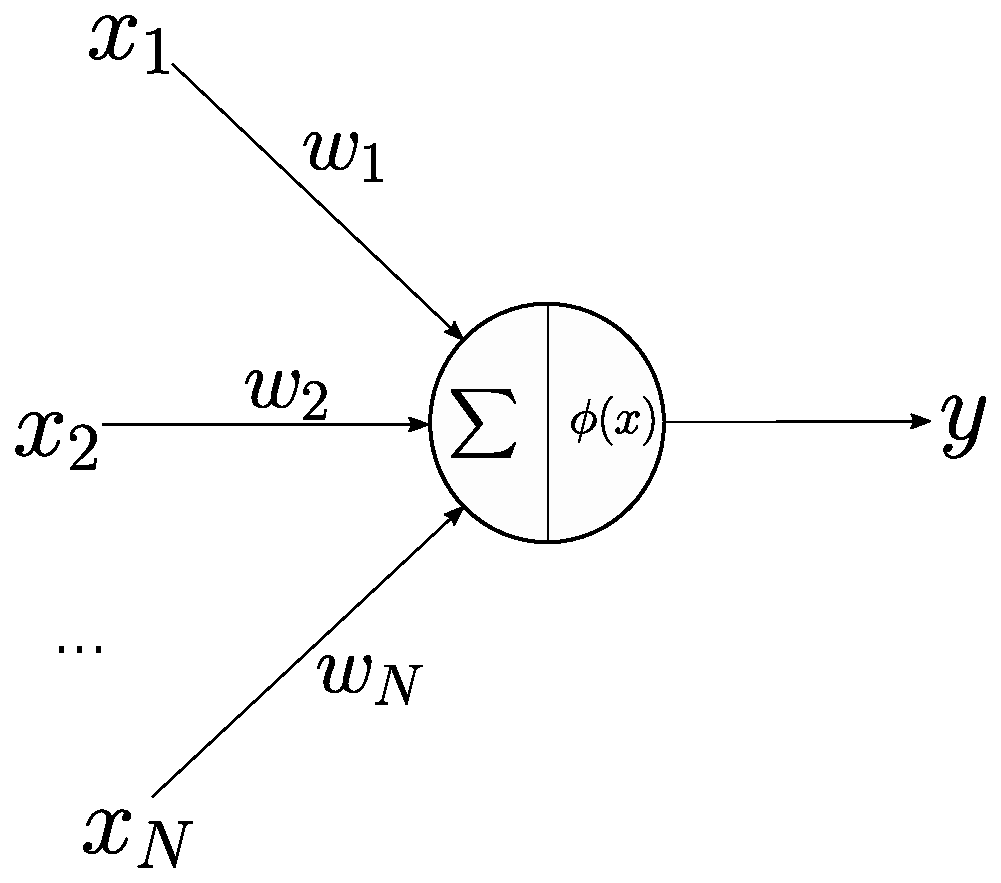
\includegraphics[width=0.5\textwidth]{perceptron-2}
	\caption{Schematischer Aufbau Neuron}
	% \todo{Quelle Bild!}
	\label{fig:singleNeuron}
\end{figure}

Wie in Abbildung~\ref{fig:singleNeuron} zu sehen haben die einzelnen Eingaben \(x_i\) jeweils eine Gewichtung \(w_i\).
Es existiert ein Schwellwert oder \textit{bias}, der normalerweise 
durch eine zusätzliche Eingabe \(x_{m+1}\) mit dem Wert \(+1\) und dem dazugehörigen Gewicht \(w_{m+1}\) modelliert wird.
Den Ausgabewert \(y\) erhält man dadurch, dass man die gewichteten Eingaben aufsummiert und in die Aktivierungsfunktion \( \phi \) des Perzeptrons gibt.
Mathematisch ist die Ausgabe eines Perzeptrons also wie folgt definiert:

\begin{equation}
	y = \phi \Big( \sum_{i= 0}^{m} w_i x_i \Big)
\end{equation}

Ein Überblick über verschiedene Aktivierungsfunktionen, die für solch ein Perzeptron benutzt werden, ist unter~\ref{sec:activationfuncs} zu finden.
Beim Lernen werden die Gewichte der einzelnen Eingaben so an gepasst, dass die gewünschte Ausgabe erreicht wird.
\todo{Vielleicht ein paar Sätze zum Perceptron Learning Algorithm?}
Ein einzelnes Perzeptron mit zwei Eingängen kann zur Darstellung der logischen Operatoren AND, OR und NOT genutzt werden

% Letztendlich ist ein solches Perzeptron jedoch nur ein linearer Klassifikator und kann somit 
% zum Beispiel den XOR Operator nicht auflösen.
Ein Perzeptron ist jedoch nur ein linearer Klassifikator und kann dementsprechend zum Beispiel den XOR Operator nicht korrekt abbilden.
Dies zeigten Marvin Minksy und Seymour Papert 1969 in einflussreichen Buch \textit{Perceptrons: an introduction to computational geometry} \todo{quelle}
\todo{Linear Trennbares / Nicht-linear Trennbares Problem (AND vs XOR)}

Solche, nicht linear-separierbare Probleme zu lösen müssen mehrere Schichten an Neuronen kombiniert werden.

\subsection{Aktivierungsfunktionen}
\label{sec:activationfuncs}
\todo[inline]{Entscheiden, ob diese Section weg soll, oder auf nur ReLU reduziert werden sollte}
Es gibt verschiedene Aktivierungsfunktionen, die für den Einsatz in neuronalen Netzen in Frage kommen.
Sie sind von notwendig, da ohne eine Nicht-Linearität das Netz in eine einfache Regression kollabiert.

Eine Aktivierungsfunktion sollte leicht abzuleiten sein, 
da dies im Rahmen des Trainings mit dem Backpropagation Algorithmus häufig geschieht 
und sonst beträchtlicher Rechenaufwand entsteht.
\todo[inline]{das referenziert dinge von Backprop, die der Leser hier vielleicht noch gar nicht weiß - Nach hinten?}

In der Vergangenheit wurden einige verschiedene Aktivierungsfunktionen verwendet.
% Einige häufig verwendete Aktivierungsfunktionen sollen hier vorgestellt werden.
Jede dieser Funktionen stellt eine Nicht-Linearität dar und nimmt eine einzelne Zahl, wendet eine bestimmte, festgelegte mathematische 
Operation auf diese an und gibt das Ergebnis zurück.
Historisch ist häufig die Sigmoid-Funktion verwendet worden, da sie das Verhalten eines natürlichen Neurons gut nachbildet.
\begin{equation}
	f(x) = \frac{1}{1 + e^x} = \frac{e^x}{e^{x + 1}}
	\label{func:Sigmoid}
\end{equation}
In der Praxis jedoch haben sich einige Nachteile der Sigmoid-Funktion gezeigt.
\todo{hier noch genauer drauf eingehen?}
Einige dieser Probleme konnten mit der Verwendung des Tangens hyperbolicus (tanh) behoben werden, 
durchgesetzt haben sich jedoch in letzter Zeit sogenannte \textit{Rectified Linear Units}, oder kurz ReLUs.

% \begin{description}
	
	% hier Könnte man die Absätze zu Sigmoid und TanH einfügen
	% \item[Sigmoid-Funktion] \hfill \\
		\begin{equation}
			f(x) = \frac{1}{1 + e^x} = \frac{e^x}{e^{x + 1}}
			\label{func:Sigmoid}
		\end{equation}
		\begin{equation}
			f'(x) = f(x) * (1 - f(x))
		\end{equation}
		Die mathematische Form der Sigmoid Aktivierungsfunktion ist in Abbildung \ref{sigmoidFunc} zu sehen.
		Sie bildet die reellen Zahlen \(\mathbb{R}\) auf das Intervall \((0,1)\) ab. 
		Für betragsmäßig größer werdende negative Zahlen nähert sich der Rückgabewert \(0\) an,
		ebenso wie für größer werdende positive Zahlen sich der Rückgabewert an \(1\) annähert.

		Die Sigmoid Funktion ist eine historisch häufig genutze Funktion, da sie das Verhalten eines natürlichen Neurons,
		der biologischen Motivation für künstliche Neuronen, gut nachbildet:
		komplette Inaktivität eines Neurons bei Ausgabe 0 bis zum feuern mit maximaler Frequenz bei Ausgabe 1.

		In der Praxis jedoch haben sich einige Nachteile der Sigmoid Funktion gezeigt, weshalb sie quasi nicht mehr genutzt wird.
		Der gewichtigste von diesen ist, dass ihre Ableitung bei großen Beträgen beinah \(0\) ist.
		Dies führt dazu, dass während der Ausführung des Backpropagation-Algorithmus beinah keine Änderungen passieren und dementsprechend das Netz sehr langsam lernt.
		
		\begin{figure}
			\centering
			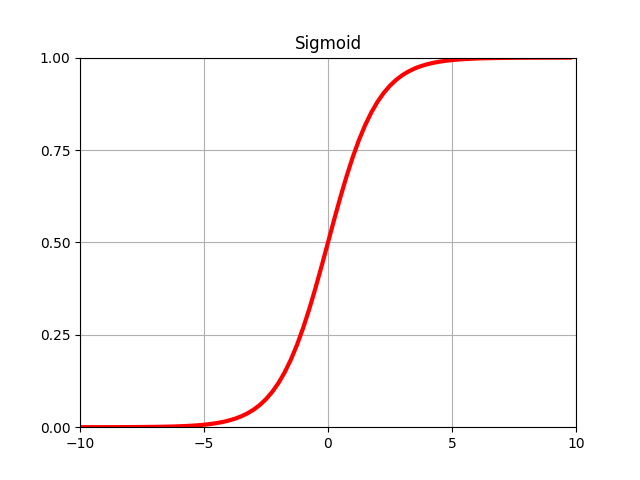
\includegraphics[width=0.618\textwidth]{Sigmoid}
			\caption{Plot der Sigmoid Funktion}
			\label{sigmoidFunc}
		\end{figure}
		  


	\item[TanH] \hfill \\
		\begin{equation}
			f(x) = \tanh(x) = \frac{e^x - e^{-x}}{e^x + e^{-x}}
		\end{equation}
		\begin{equation}
			f'(x) = 1 - f(x)^2
		\end{equation}
		Die TanH-Aktivierungsfunktion ist in Abbildung \ref{tanhfunction} dargestellt.
		Im Gegensatz zur Sigmoid Funktion bildet sie die reellen Zahlen \(\mathbb{R}\) auf das Intervall \((-1, 1)\) ab.
		Weil sie zentriert um den Nullpunkt ist, wird sie bei realen Anwendungen der Sigmoid Funktion vorgezogen.
		Das Saturationsproblem der Sigmoid Funktion besteht jedoch immer noch.
		\begin{figure}
			\centering
			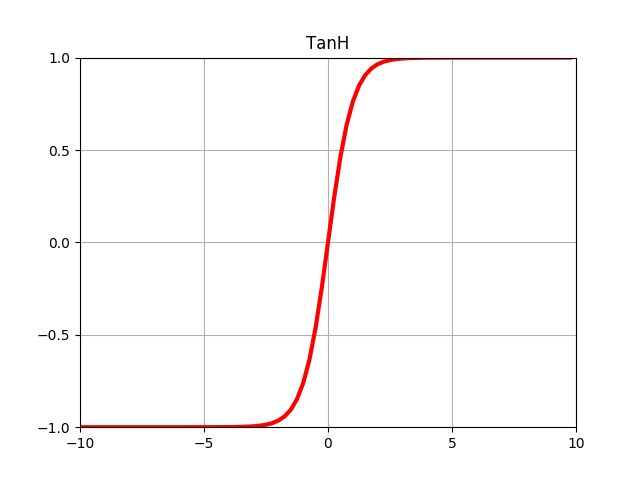
\includegraphics[width=0.618\textwidth]{Tanh}
			\caption{Plot der Tanh Funktion}
			\label{tanhfunction}
		\end{figure}
	
	% \item[ReLU] \hfill \\
\begin{equation}
	f(x) = \max(0, x)
\end{equation}
\begin{equation*}
	f'(x) = \begin{cases}
	0 &\text{, falls $x < 0$}\\
	1 &\text{, falls $x > 0$}
	\end{cases}
\end{equation*}
	Abbildung~\ref{reluoutput} zeigt das Schaubild einer solchen ReLU. 
	\todo{ReLU plot neu machen: dicker bei unter 0 und als Vector graphic statt als PNG}
	Die Aktivierung von ReLUs ist ein einfacher Schwellwert, der weit weniger rechenintensiv ist, als die aufwendigen Exponenzialfunktionen von Sigmoid und tanh.
	In der Praxis hat sich gezeigt zudem gezeigt, dass ReLus deutlich schneller konvergieren als Sigmoid- oder tanh-Neuronen.  
	Krizhevsky et al. haben in ihrem Paper~\cite{NIPS2012_4824} einen Geschwindigkeitsgewinn um Faktor 6 feststellen können.
	Ein Problem, das mit ReLUs jedoch existiert ist, dass einzelne Neuronen während dem Training "absterben" können, falls sie irgendwann in dem Bereich landen, wo der Gradient 0 ist.
	Diese Neuronen sind dann für jeden beliebigen Input inaktiv und können niemals wieder etwas zur Ausgabe des Netzes beitragen.
	Durch die Wahl einer geeigneten Lernrate oder den Einsatz sogenannter Leaky ReLUs lässt sich dies jedoch vermeiden.
	Leaky ReLUs haben im Gegensatz zu normalen ReLUs eine kleine positive Steigung im negativen Bereich.
	\begin{equation}
		f(x) = \begin{cases}
			x &\text{, falls } x  >  0\\
			0.01 x &\text{, falls } x  \leq  0
		\end{cases}
	\end{equation} 
	

	\begin{figure}[h]
		\centering
		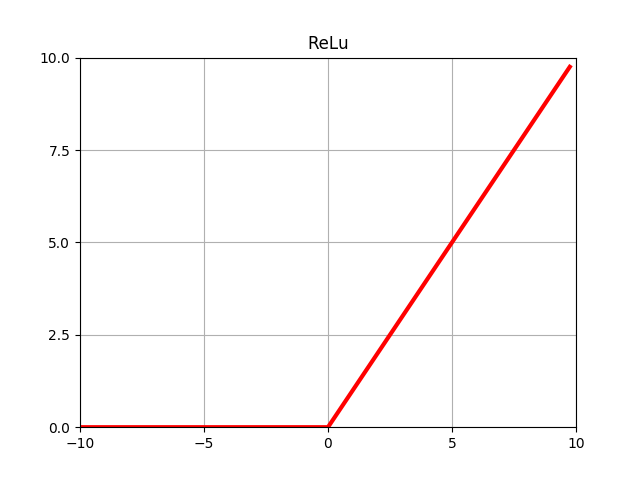
\includegraphics[width=0.618\textwidth]{ReLu}
		\caption{Schaubild der Ausgabe einer ReLU}
		\label{reluoutput}
	\end{figure}



% \end{description}

% \begin{figure}[h]
%     \centering
%     \begin{subfigure}[t]{0.3\textwidth}
% 		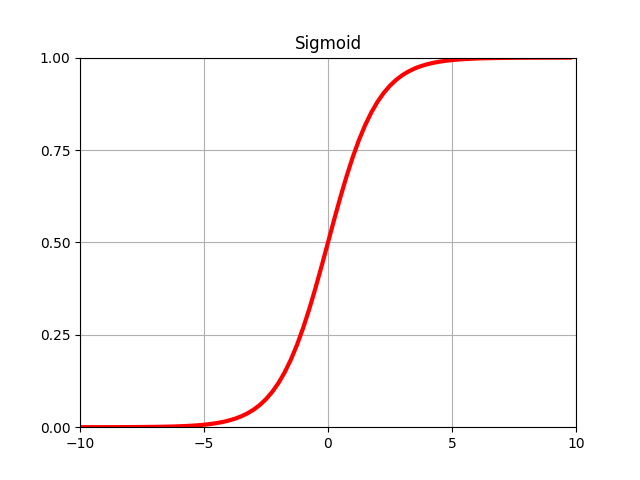
\includegraphics[width=\textwidth]{Sigmoid}
% 		\caption{Sigmoid Funktion}
%     \end{subfigure}
%     \begin{subfigure}[t]{0.3\textwidth}
% 		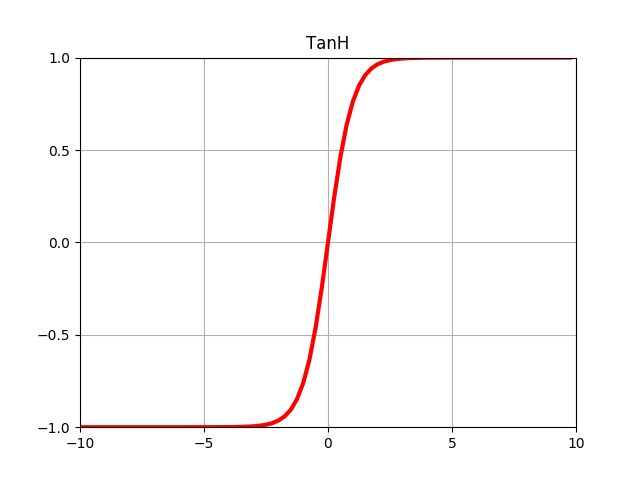
\includegraphics[width=\textwidth]{Tanh}
% 		\caption{TanH Funktion}
%     \end{subfigure}
%     \begin{subfigure}[t]{0.3\textwidth}
%         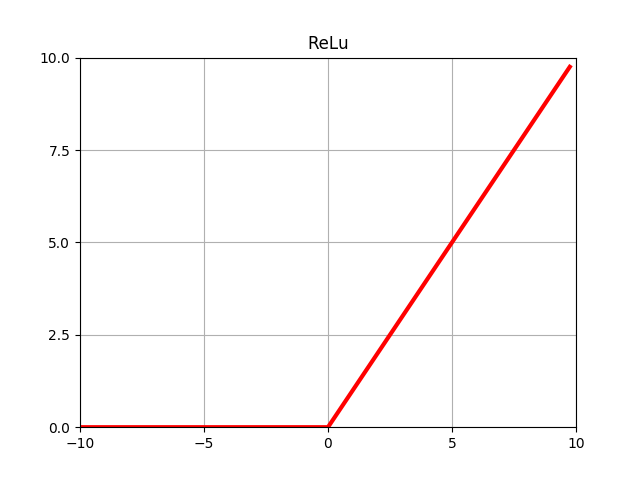
\includegraphics[width=\textwidth]{ReLu}
%         \caption{ReLU}
%     \end{subfigure}
%     \caption{Häufig verwendete Aktivierungsfunktionen}
%     \label{eval:function}
% \end{figure}



\subsection{Feedforward Netze}

% \textbf{absatz über Feedforward Netze. Basic}
\begin{itemize}
	\item Definition (keine Kreise oder Schleifen). (Kommentar Florian: \"Rückkopplung\")
	\item Gegenstück zum RNN
	\item grundlegende Architektur in Layern 
	\item Aktivierungsfunktionen in Layern
	\item Outputlayer: Verschiedene Aktivierungsfunktionen:
	\item Linear für regression, z.B. Softmax für Wahrscheinlichkeitsverteilung Softmax
\end{itemize}



Als Feedforward Netz bezeichnet man ein neuronales Netz, zwischen dessen Knoten keine Kreise oder Schleifen existieren.
Ein Netz in dem es solche Verbindungen gibt bezeichnet man als \textit{Rekurrentes Neuronales Netz}.
Die Informationen wandert in der Verarbeitungsrichtung von den Eingabeknoten zu den Ausgabeknoten.
Für gewöhnlich sind die einzelnen Knoten in Schichten, sogenannten Layern, organisiert.
Die Neuronen eines einzelnen Layers sind meist 
Die Eingabe wird in ein Input Layer eingeben.

\subsection{Backpropagation}

\todo[inline]{Optional: am Ende entscheiden ob ich noch mehr Kontent möchte und dann gegebenenfalls ausformulieren}
Der Backpropagation Algorithmus ist ein Verfahren mit denen künstliche neuronale Netze in der Lage sind komplizierte Zielfunktionen einzulernen.
Es ist eine Methode, bei der effizient der Gradient der Fehlerfunktion in Abhängigkeit vom Gewicht der einzelnen Kanten im Netz bestimmt werden kann,
was dann für einen Gradientenabstieg verwendet werden kann. 

\color{blue}
\begin{itemize}
	\item Definition und Beschreibung
	\item Nur supervised learning: Gradient der Fehlerfunktion wird benötigt \(\rightarrow\) Tatsächliches Ergebnis muss bekannt sein.
	\item "Finden einer Funktion, die am besten die Inputs auf die outputs mapt"
\end{itemize}
\color{black}

\subsection{Performancemaß}

Das essenzielle Maß nachdenen neuronale Netze bewertet werden, ist wie gut sie mit neuen, unbekannten Daten umgehen, die nicht in den Trainingsdaten vorhanden waren. 
Diese Eigenschaft von Trainingsdaten auf unabhängige Testdaten zu schließen wird Generalisierung genannt. 

Als Overfitting bezeichnet man es, wenn ein Modell sich zu sehr an ein gegebenes Datenset anpasst und 
dafür in Kauf nimmt zusätzliche oder zukünftige Daten schlechter zu repräsentieren.
Das System wird also schlechter darin zu generalisieren.

Im Feld des überwachten Lernens beziehungsweise der neuronalen Netze ist Overfitting daran zu erkennen,
dass die Qualität die Ausgaben des Netzes auf dem Trainingsdatenset sich weiter verbessert,
während sie auf dem Testdatenset schlechter wird.
Dies kann zum Beispiel der Fall sein, wenn das Modell Rauschen in den Testdaten als Teil der zugrundeliegenden Struktur interpretiert. 


Dem Overfitting gegenüber steht das Underfitting. 
Als Underfitting bezeichnet man wenn das Netz nicht in der Lage ist
eine ausreichend gute Performance auf den Trainingsdaten zu erreichen.
Das kann passieren wenn das Modell nicht ausreichend komplex ist um die zugrundeliegende Struktur der Daten abzubilden.


Sowohl Overfitting als auch Underfitting hängen mit der Kapazität eines Netzes zusammen.
Ist die Kapazität zu gering kann es sein, dass das Netz daran scheitert die Trainingsdaten zu lernen.
Ist die Kapazität zu groß, so kann es passieren, dass das Netz, umgangsprachlich ausgedrückt, die Trainingsdaten einfach auswendig lernt.
\todo{umgangsprachlich mit einer besseren Formulierung ersetzen...}

Dies ist beispielhaft in Abbildung~\ref{fig:capacity} zu sehen.
Aus der zugrundeliegenden \( \cos \)-Funktion werden Stichproben mit einem Rauschterm entnommen. 
Stellvertretend für das Lernen mit neuronalen Netzen wird hier lineare Regression benutzt,
um die Parameter eines Polynoms zu lernen.
Die Kapazität des Modells wird hier durch den Grad des Polynoms festgelegt.

In Abbildung~\ref{subfig:underfitting} wird ein Polynom mit dem Grad 1 gelernt.
Die Kapazität ist zu niedrig und dementsprechend schafft das Modell es nicht die Stichproben akkurat zu repräsentieren.

In Abbildung~\ref{subfig:rightfitting} ist der Grad des Polynoms 4.
Das resultierende Modell ist eine gute Approximation der ursprünglichen Funktion.

In Abbildung~\ref{subfig:overfitting}

\begin{figure}[h]
    \centering
	
	\begin{subfigure}[t]{0.6\textwidth}
		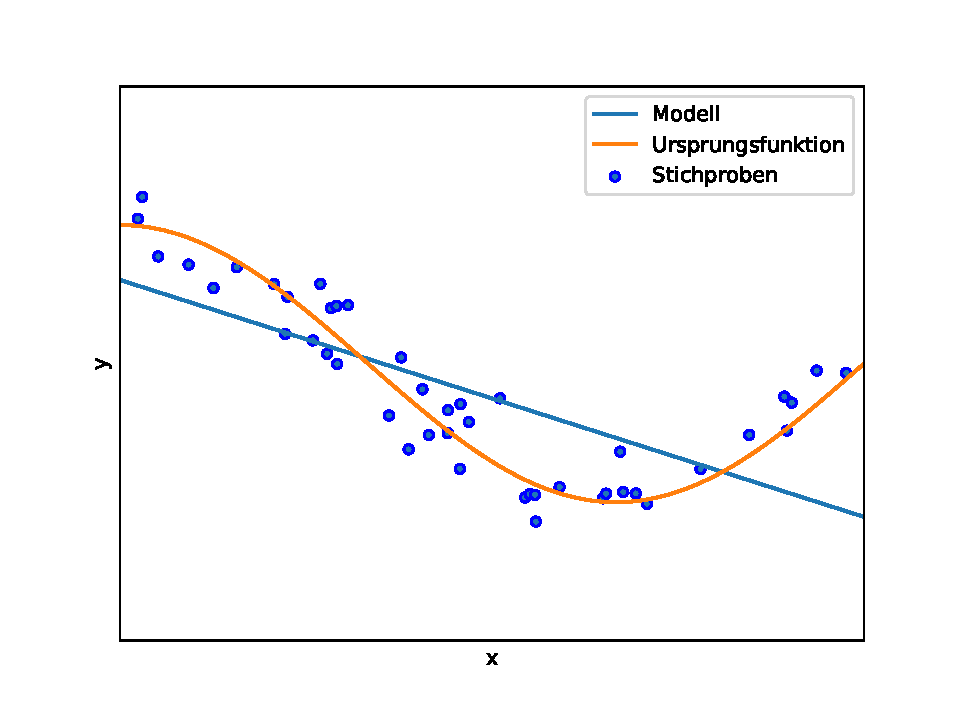
\includegraphics[width=\textwidth]{plotUnderfitting.pdf}
		\caption{Underfitting}
		\label{subfig:underfitting}
	\end{subfigure}
	% \quad
	\begin{subfigure}[t]{0.6\textwidth}
		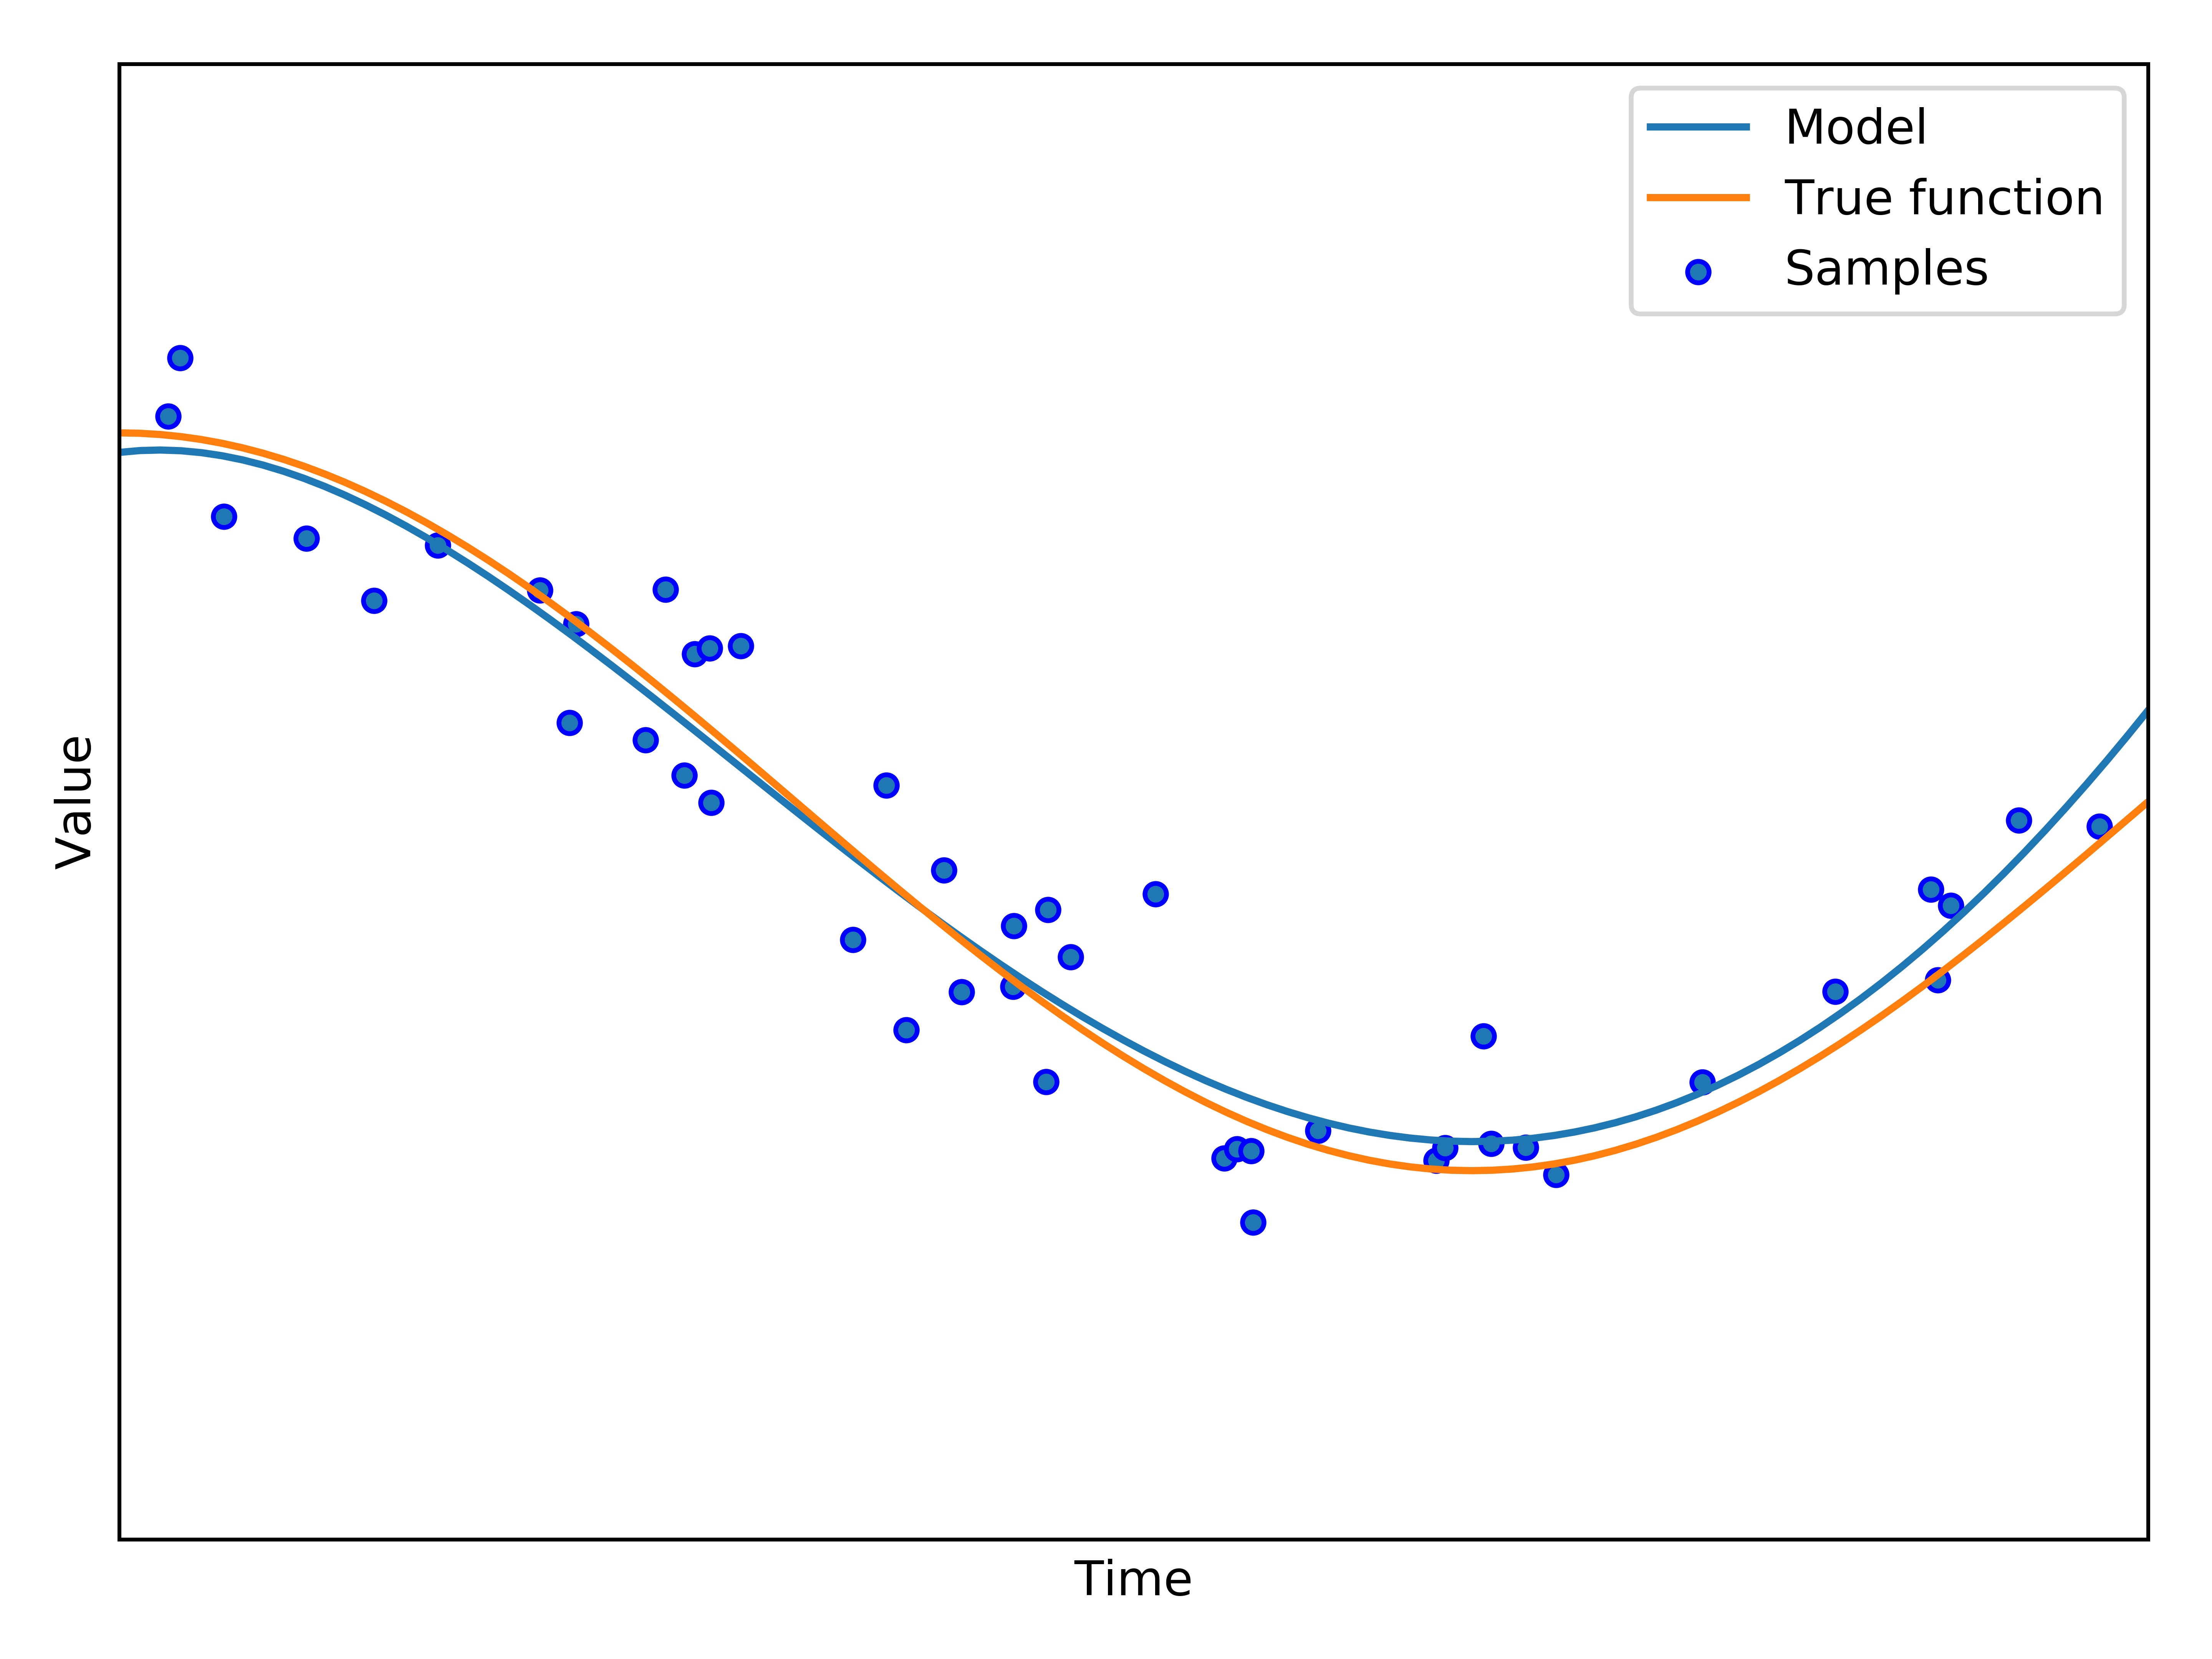
\includegraphics[width=\textwidth]{plotPassendesModell.pdf}
		\caption{Passendes Modell}
		\label{subfig:rightfitting}
	\end{subfigure}
	% \quad
	\begin{subfigure}[t]{0.6\textwidth}
        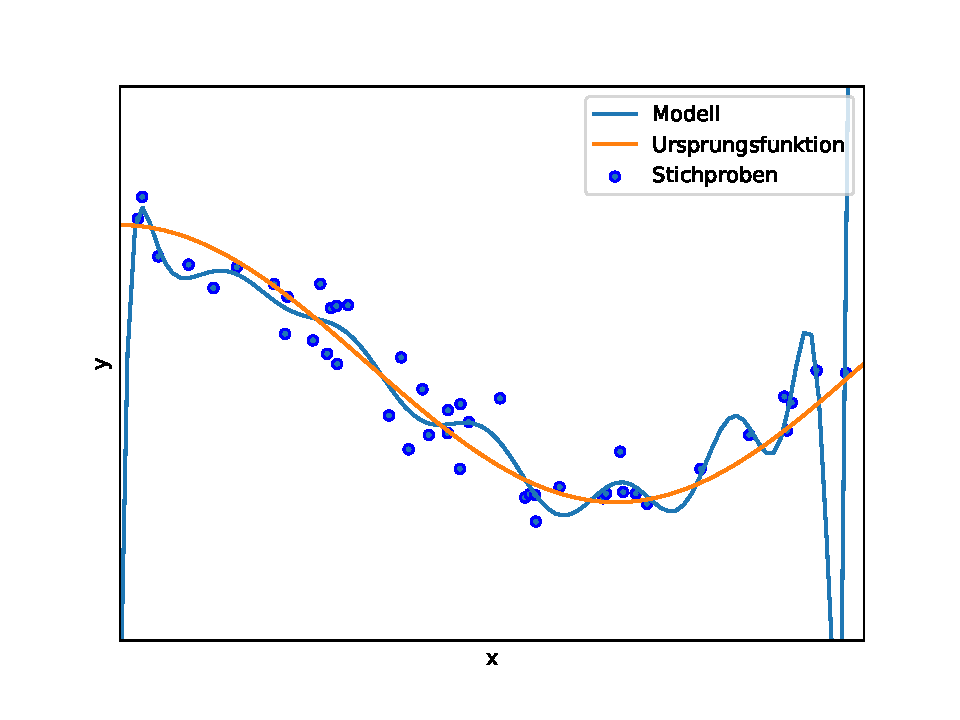
\includegraphics[width=\textwidth]{plotOverfitting.pdf}
		\caption{Overfitting}
		\label{subfig:overfitting}
	\end{subfigure}
	\caption{Visualisierung von unterschiedliche Kapazitäten}
	\label{fig:capacity}
\end{figure}

\begin{itemize}
	\item Methoden um Overfitting zu vermeiden:
	\item Mehr Trainingsdaten (z.\,B. durch Data-Augmentation)
	\item Regularisierung (L1, \(L_2\) (siehe unten), dropout)
\end{itemize}


\subsection{Regularisierung} \label{ssec:Regul}

\color{blue}
\begin{itemize}
	\item Regularisierung Definition
	\item Mathematische Formel Darstellung
	\item \(L_1\) und \(L_2\) Regularisierung
	\item L0 - warum nicht?
	\item (Maybe Dropout)
	\item Early Stopping? (das internet sagt, es ist eine art von Regularisierung und falls ich sie verwenden sollte, sollte ich sie hier erwähnen)
\end{itemize}
\color{black}

Als Regularisierung bezeichnet man eine Technik, die zur Vermeidung von Overfitting verwendet wird.
Sie wird in der Hoffnung angewendet, dass das Modell mit Regularisierung besser generalisiert als ohne.

Eine Möglichkeit ist, dass zur Loss Funktion ein Regularisierungsterm \(R\) hinzugefügt wird, 
der die Kosten basierend auf der Komplexität des Systems erhöht.

\begin{equation}
	\min_f \sum\limits_{i=1}^{m} V(f(\vec{x}_i), \vec{y}_i) + \lambda R(f)
\end{equation} 

Dabei ist \(V\) die Loss Funktion, beispielsweise \textit{Mean-Square-Error} oder \textit{Mean-Absolute-Error}.
\(n\) ist die Anzahl der Feature-Label-Paare,
\(x_i\) und \(y_i\) sind die einzelnen Eingabefeatures und das dazugehörige Label.
Die Funktion \(f\) ist in unserem Fall das neuronale Netz, das die Features entgegen nimmt.
\(\lambda\) ist ein Parameter, der die Gewichtung des Regularisierungsterm festlegt.
Wählt man diesen Parameter zu klein, so kann es sein, dass das Modell trotz Regularisierung noch immer overfittet.
Wählt man ihn zu groß so kann es sein, dass das Modell das Problem nicht mehr korrekt abbildet und es zu Underfitting kommt.
Der Regularisierungsterm \(R\) wird so gewählt, dass er die Komplexität der Funktion \(f\) wiederspiegelt.
Ein gutes Maß für die Komplexität eines neuronalen Netzes sind die Gewichte zwischen den Neuronen.
Beispiele für \(R\) wären zum Beispiel die \(L_1\)- oder die \(L_2\)-Regularisierung. % die jeweils mit der \(L_1\) beziehungsweise mit der \(L_2\)-Norm arbeiten.
Der entscheidende Unterschied zwischen den beiden ist der unterschiedliche Strafterm, zu sehen in~\ref{eqn:MSE-L1} für \(L_1\) und~\ref{eqn:MSE-L2} für \(L_2\). 
Die Fehlerfunktionen sind jeweils MSE mit dazugehörigen Strafterm.

\begin{equation} \label{eqn:MSE-L1}
	J(X, Y) = \frac{1}{m} \sum_{i=1}^{m} (\vec{y}^{(i)} - \hat{\vec{y}}^{(i)})^2 + \sum_{j, k} (|\mat{W}_{j,k}|)
\end{equation} 

\begin{equation} \label{eqn:MSE-L2}
	J(X, Y) = \frac{1}{m} \sum_{i=1}^{m} (\vec{y}^{(i)} - \hat{\vec{y}}^{(i)})^2 + \sum_{j, k} (\mat{W}_{j,k}^2)
\end{equation} 


Ein Regressionsmodell, dass \(L_1\)-Regularisierung verwendet wird auch als Lasso Regression bezeichnet, 
während ein Modell mit \(L_2\)-Regularisierung als Ridge Regression beschrieben werden kann.
Vergleicht man die beiden Ansätze, so schrumpft die \(L_1\) Norm weniger wichtige Gewichte auf 0, was zu dünn besetzten Gewichtsvektoren führt.
Dies kann eine wünschenswerte Eigenschaft sein.
Im Gegensatz dazu hat die \(L_2\)-Regularisierung, den Vorteil, dass sie effizienter berechnen kann.
Der Strafterm von \(L_2\) hat eine geschlossene Form und kann in Form einer Matrix angewendet werden, während die Funktion von \(L_1\) auf Grund des Betrags eine nicht-differenzierbar ist.


\todo{absatz zu (L0 und warum man es nicht benutzt?)}

Eine weitere Regularisierungstechnik ist Dropout~\cite{JMLR:v15:srivastava14a}.
Dabei werden während dem Training eines neuronalen Netzes 
mit einer festgelegten Wahrscheinlichkeit zufällig Neuronen und die dazugehörigen Verbindungen abgeschaltet, 
wie in Abbildung~\ref{fig:dropout} dargestellt.
\todo{Ist die Grafik essenziell fürs Verständnis?}
Dies soll insofern Overfitting vermeiden, dass es übermässige Kodaption von mehreren Neuronen erschwert.
Dropout als Technik wird insbesondere bei tiefen neuronalen Netzen eingesetzt. 

\begin{figure}[h]
    \centering
    \begin{subfigure}[t]{0.4\textwidth}
		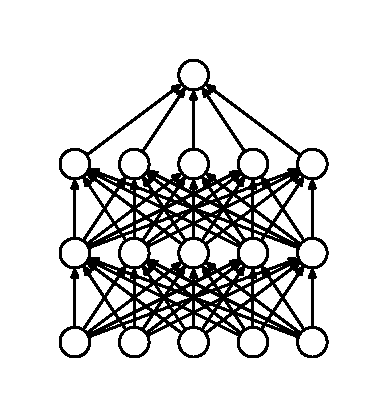
\includegraphics[width=\textwidth]{neuralNet}
		\caption{Unverändertes neuronales Netz}
    \end{subfigure}
    \begin{subfigure}[t]{0.4\textwidth}
		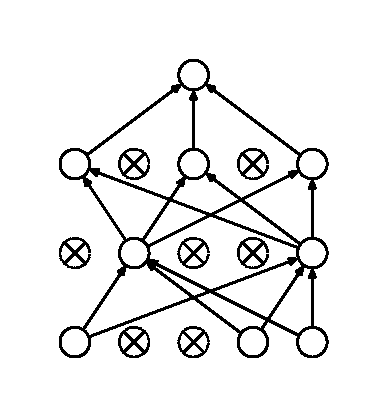
\includegraphics[width=\textwidth]{neuralNet_dropped}
		\caption{Nach Dropout Anwendungen.}
	\end{subfigure}
    \caption{Beispiel Dropout-Regularisierung~\cite{JMLR:v15:srivastava14a}}
    \label{fig:dropout}
\end{figure}


\section{TableSort System}

\todo[inline]{Viel stuff über das TableSort System}

\begin{itemize}
	\item kleiner, experimenteller Bandsortierer~\cite{doll2015}
	\item Entstanden in Kooperation zwischen dem Fraunhofer IOSB, Abteilung Sichtprüfsysteme, und dem Institut für Intelligente Sensor Aktor Systeme des Karlsruher Institut für Technologie.
	\item Im Rahmen des \textit{TrackSort} Projekts
	\item Gedacht für Experimente, wenn es zu aufwendig ist das mit dem großen großen zu machen und zum Mitnehmen auf Messen.
	\item 2 Modi: mit Förderband und mit Rutsche
	\item Mit Flächenkamera für TrackSort als auch die Zeilenkamera sind dargestellt.
	\item Ringlicht (Refence später)
	\item Die Zeilenkamera wird zurzeit in industriellen Schüttgutsortieranlagen verwendet, ist aber nicht optimal (Siehe all die Literatur)
\end{itemize}

Das Table

\begin{figure}[h]
	% \missingfigure{Bild von TablesortSystem}
	\includegraphics[width=\textwidth]{TrackSortPic}
	\caption{TableSort Schüttgutsortiersystem \cite{fraunhoferiosb2017}}
	% \todo{Quelle Bild!}
	\label{fig:tablesortsystem}
\end{figure}


\begin{figure}[h]
    \centering
    \def\svgwidth{\columnwidth}
	\input{img/Aufbau-moved.pdf_tex}
	\label{fig:aufbau_tablesort}
	\caption{Schematische Darstellung des optischen Bandsortierers TableSort nach~\cite{Pfaff2017}.}
\end{figure}



    \section{Stand der Technik}
\label{cap:relWork}

Notizen:
\todo[inline]{Das aller aller dickste TODO}
\color{blue}
Wie wird das, was ich dann mit Neuronalen Netzen machen möchte aktuell gemacht?


Teilaspekt vom Tracksort Multi-Targettracking: Bewegungsprädiktion.
Primär Florian's Dissertation: Kapitel 4.


\begin{itemize}
    \item Im Rahmen dieser Arbeit es geht um die Prädiktion der Bewegung von Schüttgutpartikeln.
    \item "Bewegungsmodell" bei Zeilenkamera: Identical Delay, weil nur eine Beobachtung.
    \item Modelle erst seit Flächenkamera notwendig.
    \item Vorraussetzung: Trackassoziationen.
    \item Aber: wir nehmen dieses Problem als gelöst an.
    \item In der Realität ist es das nicht (MA Tobi K), reale daten sind nicht zwingend 100\% genau, aber wir arbeiten mal damit.
    \item in Florians Diss: mehrere Modelle beschrieben zum prädizieren:
    \item CV und CA, und was die dahinterstehenden Annahmen sind.
    \item CV: Konstante Geschwindigkeit - Perfekte Beruhigung
    \item CA: Konstante Beschleuningung - Geschwindigkeit ändert sich Konstante
    \item Dazu kommen noch Szenario spezifische Modelle, bei denen gezeigt wurden, dass sie für das Szenario besser sind.
    \item CVBC, IA - upgrades.
    \item Vorgriff ins evaluationskapitel? - dort wird dann behandelt wie man sie Mathematisch beschreibt. 
\end{itemize}

\color{black}


Im Rahmen dieser Arbeit geht es um die Prädiktion der Bewegung von Schüttgutpartikeln.
Der Einsatz von verschiedenen Bewegungsmodellen ist erst für Schüttgutsortierer mit Flächenkamera sinnvoll.
Eine Zeilenkamera liefert nur einen einzelnen Datenpunkt bezüglich Zeit und Position eines Partikels.
In~\cite{Pfaff2018} wird unter anderem ein Bewegungsmodell beschrieben, das das Verhalten eines Schüttgutsortierers mit Zeilenkamera emuliert.
Wie in schon in Abbildung~\ref{fig:predMissed} dargestellt wurde, muss angenommen werden, dass es zu keinerlei Bewegung orthogonal zur Transportrichtung kommt.
Für die Prädiktion des Zeitpunkts wird die durchschnittliche Zeit bestimmt, die ein Partikel von der Position der Zeilenkamera zur Position des Druckluftdüsenarrays benötigt 
und diese als konstanter Offset für jede Partikeldetektion angenommen.

Um den Separationsprozess durch den Einsatz von prädiktiven Tracking Methoden und Bewegungsmodellen zu verbessern ist eine Assoziation 
der beobachteten Partikelpositionen zu tatsächlichen Tracks notwendig. 
Im Rahmen dieser Arbeit wird dieses Problem nicht betrachtet. 
Es wird direkt mit den assozierten Trackdaten gearbeitet, 
obwohl dieser Assoziationsprozess noch Gegenstand aktueller Forschung ist.
\todo{hier schon erwähnen, dass die Assoziation auf den selbst gesammelten Daten vielleicht flawed ist?}

Die grundlegenden Bewegungsmodelle, die in \cite{Pfaff2018} beschrieben werden sind 
einerseits das Constant Velocity Modell und andererseits das Constant Acceleration Modell.
Das Constant Velocity Modell prädiziert die Bewegung eines Teilchens unter der Annahme, dass es sich mit einer konstanten Geschwindigkeit bewegt.
Basierend auf den letzten zwei bekannten Positionen des Partikels wird dessen Geschwindigkeit entlang der beiden Achsen bestimmt 
und davon die zukünftige Bewegung abgeleitet.
Diese Annahme ist jedoch nicht immer korrekt.
Es kann sein, dass bei einem Bandsortierer das Förderband nicht lang genug ist, um das Schüttgut komplett zu beruhigen.
Dann haben die Teilchen eine Beschleuningung, die nicht 0 ist.
Das Constant Acceleration Modell dahingegen prädiziert die Bewegung des Teilchens unter der Annahme, dass es sich mit einer konstanten Beschleuningung bewegt.
Diese Beschleuningung wird anhand der letzten drei bekannten Positionen bestimmt.
Anhang dieser Beschleuningung und der aktuellen Geschwindigkeit werden die zukünftigen Positionen abgeleitet.

In \cite{Pfaff2018} werden weitere, szenariospezifische Bewegungsmodelle beschrieben.
Bei dem sogenannten Bias-Corrected Constant Velocity Modell wird das Constant Velocity Modell als Grundlage genommen und ein Korrekturterm eingeführt.
Basierend auf den zuvor beobachteten Schüttgutpartikeln wird ein durchschnittlicher temporaler Bias bestimmt, der von den zukünftigen Prädiktionen abgezogen wird.
Die Annahme ist hier, dass der Bias von zukünftige Partikel ähnlich zu dem der zuvor beobachteten Partikeln sein wird.
Beim Identical Acceleration Modell wird ebenfalls ein Korrekturterm benutzt, 
der im Gegensatz zum Bias-Corrected Constant Velocity Modell jedoch nicht absolut, sondern abhängig von der letzten bekannten Position des Partikels ist.
Auf jedem der zuvor beobachteten Partikeln wird der Wert einer zusätzlichen Beschleuningung bestimmt, die zu einer optimalen Prädiktion führen würde und dann der Durchschnitt dieser Beschleunigungen gebildet.
Dieser wird dann als Korrekturterm auf ein Constant Velocity Modell addiert, sodass sich eine Formel ähnlich zu der des Constant Acceleration Modelles ergibt.
Um das Verhalten von den Partikeln, deren Geschwindigkeit sich der des Förderbands nähert ohne sie zu überschreiten, besser abzubilden als durch ein Constant Acceleration Modell,
wird das Constant Acceleration with Limited Velocity Modell beschrieben. 
Dabei wird die Geschwindigkeit des Förderbands bestimmt und Partikel, die diese erreichen, von dann aus mit konstanter Geschwindigkeit weiter prädiziert.
Es wurden zudem zwei Modelle, Constant Acceleration Disallowing Sign Change Modell und Ratio-Based Deceleration Modell, vorgestellt, 
die spezifisch konzipiert wurden um die Bewegungprädiktion orthogonal zur Transportrichtung zu verbessern.


    \chapter{Datenverarbeitung}

% Wie bei jeder Anwendung von maschinellen Lernverfahren sind die zugrundeliegenden Daten von äußerster Wichtigkeit.
Bei maschinellen Lernverfahren ist die Qualität und die Menge der zugrundeliegenden Daten sehr wichtig,
da diese die Güte des Ergebnisses stark beeinflussen können.
Im Rahmen dieser Masterarbeit wurden zweierlei Arten von Daten benutzt:
Einerseits wurden am \textit{TableSort} Schüttgutsortierer des Fraunhofer IOSBs Aufnahmen gemacht, 
die dann über mehrere Arbeitsschritte in das richtige Datenformat übersetzt wurden.
Zudem existieren Datensätze, die durch eine Simulation mittels der \textit{Diskrete-Elemente-Methode} (DEM) entstanden sind. 
In diesem Kapitel soll nun beschrieben werden, woher diese Daten kommen, wie sie verarbeitet werden 
und in welcher Form sie dann letztendlich in die neuronalen Netze gegeben werden.
Abschließend wird die Datenaugmentierung, die vorgenommen wurde, vorgestellt und erklärt.





\section{Eigene Aufnahmen}

In diesem Abschnitt soll beschrieben werden, welche Form die am Fraunhofer IOSB selbst aufgenommenen Daten haben und welche Konfigurationen bezüglich Schüttgut und Sortierer sie darstellen.


% \subsection{Versuchsaufbau}
% \todo[inline]{passendere überschrift finden?}

% \color{blue}
% \begin{itemize}
% 	\item Am TableSort System, einmal Band, einmal Rutsche
% 	\item Beschreibung von der Bonito Kamera, stats usw.
% 	\item Umrechengröße pixel zu mm
% 	\item Bandgeschwindigkeit
% \end{itemize}
% \color{black}


Zur Aufnahme der Daten wurde eine Bonito~CL-400~200~FPS~Kamera benutzt. 
% , die in Abbildung~\ref{pictureCam} zu sehen ist.
Diese wurde, wie in Abbildung~\ref{fig:tablesortsystem} dargestellt, oberhalb des Förderbandes beziehungsweise der Rutsche angebracht.
Die Bilder, die von der Kamera aufgenommen werden, haben eine Auflösung von 2320x1726~Pixeln~\cite{alliedvisiontechnologiesgmbh2014}.
Anhand mehrerer Kalibrierungsbilder wurde bestimmt, dass 1 Pixel im Bild ungefähr \SI{0.056}{\milli\meter} entspricht.
Im weiteren Verlauf der Arbeit wird mit Pixeln~(px) als der Einheit des Orts für die selbst aufgenommenen Bilder gearbeitet.

% \todo[inline]{Rutschenkonfiguration Tablesort ausführlicher erwähnen?}
% \todo[inline]{Umrechengröße pixel zu mm, im weiteren verlauf werden pixel benutzt}

% \begin{figure}[h]
%     \centering
%     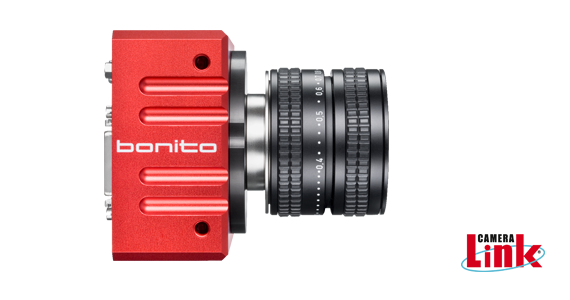
\includegraphics[width=\textwidth]{img/banner-Bonito_cropped}
%     \caption{Zur Aufnahme verwendete Kamera [TODO: Quelle Bild]}
%     \label{pictureCam}
% \end{figure}

% \subsection{Schüttgüter-Typen}

Aufgenommen wurden Daten von vier verschiedenen Schüttgütern: Kugeln, grüne Pfefferkörner, Zylinder und Weizenkörner.
Diese Schüttgüter sind in Abbildung~\ref{fig:schuettgueterSchuessel} in Schüsseln 
und in Abbildung~\ref{fig:schuettgueterBand} während den Aufnahmen zu sehen.

% die in Abbildung~\ref{fig:schuettgueterSchuessel} zu sehen sind.

% \begin{itemize}
%     \item Kugeln
%     \item grüne Pfefferkörner
%     \item Zylinder
%     \item Weizenkörner
% \end{itemize}

Die Kugeln bestehen aus Holz und haben einen Durchmesser von \SI{5}{\milli\metre}.
Die Zylinder bestehen ebenfalls aus Holz. Sie haben eine Länge von \SI{1}{\centi\metre} und einen Durchmesser von \SI{3}{\milli\metre}.
Die Kugeln und der Pfeffer, sowie die Zylinder und die Weizenkörner, bilden jeweils 
ein Paar aus einem geometrischen Körper und einem echten Objekt, das grob dessen Form ähnelt.

% \todo{Mehr Details?}

Alle Schüttgüter wurden auf der Förderbandkonfiguration des \textit{TableSort} Systems aufgenommen.
Zusätzlich dazu wurden Kugeln und Pfefferkörner auf der Rutschenkonfiguration des \textit{TableSort} Systems aufgenommen.

\begin{figure}[h]
	\centering
	\begin{subfigure}[t]{0.4\textwidth}
		\includegraphics[width=\textwidth]{KugelnCropped}
		\caption{Kugeln}
	\end{subfigure}
	\quad
	\begin{subfigure}[t]{0.4\textwidth}
		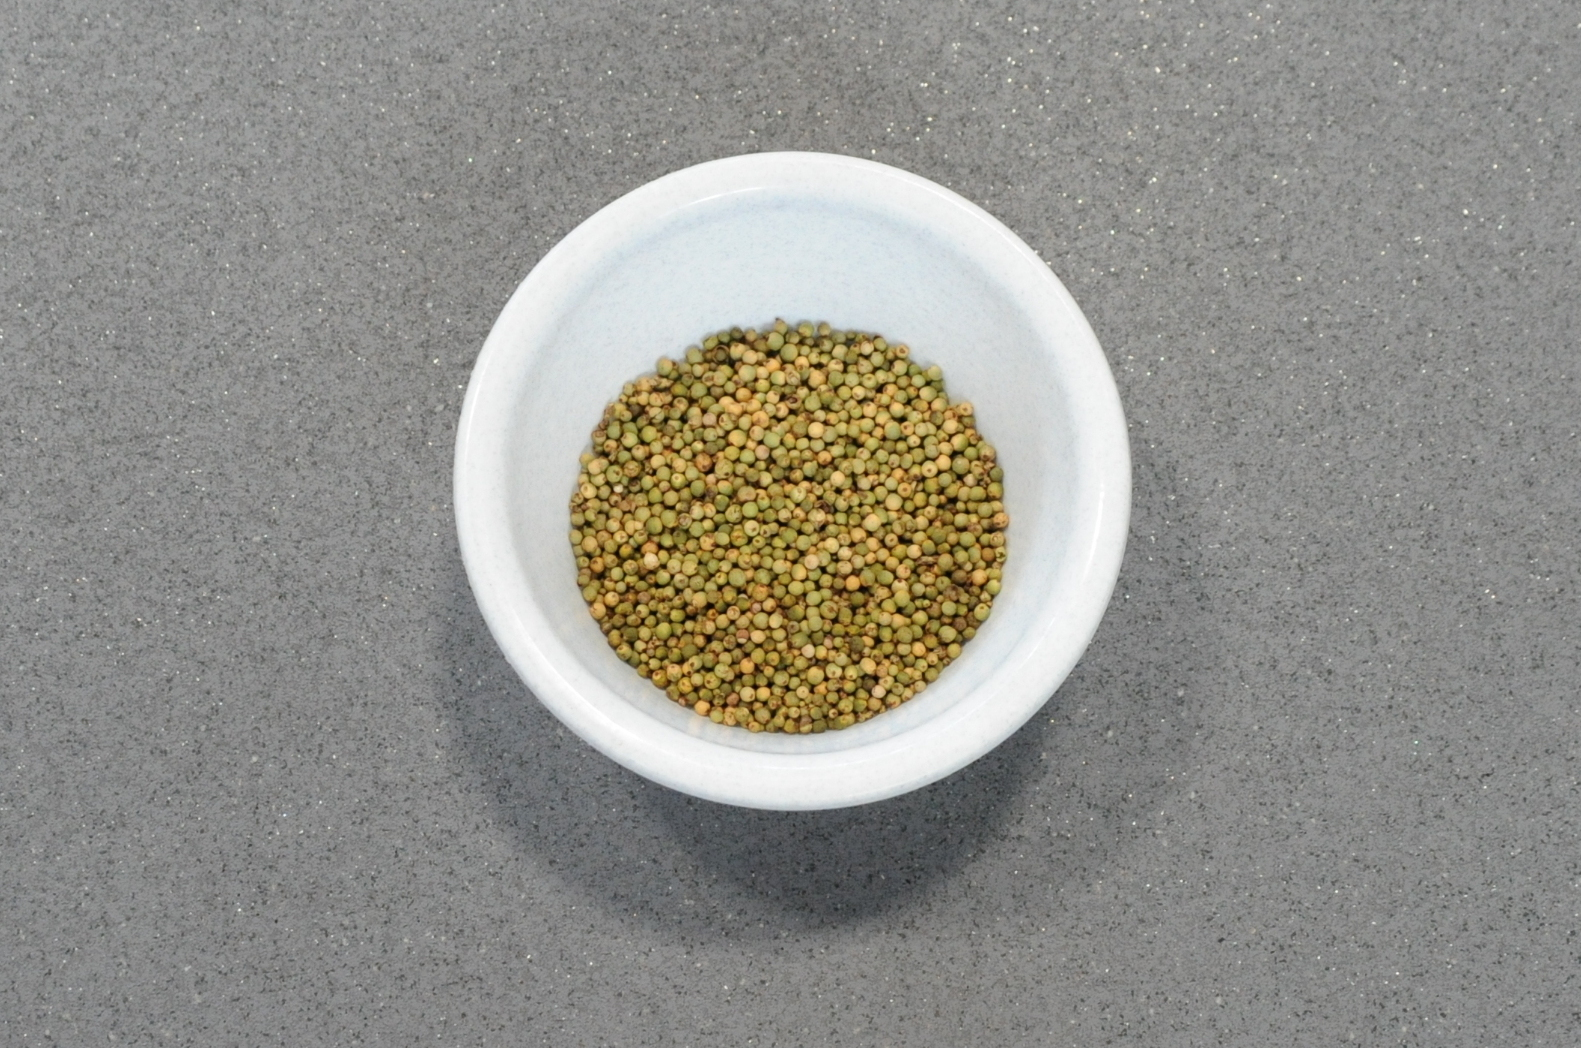
\includegraphics[width=\textwidth]{PfefferCropped}
		\caption{Pfefferkörner}
	\end{subfigure}
	\vskip\baselineskip
	\begin{subfigure}[t]{0.4\textwidth}
		\includegraphics[width=\textwidth]{ZylinderCropped}
		\caption{Zylinder}
	\end{subfigure}
	\quad
	\begin{subfigure}[t]{0.4\textwidth}
		\includegraphics[width=\textwidth]{WeizenCropped}
		\caption{Weizen}
	\end{subfigure}
	\caption{Verschiedene gesammelte Schüttgüter}
	\label{fig:schuettgueterSchuessel}
\end{figure}

\begin{figure}[h]
	\centering
	\begin{subfigure}[t]{0.4\textwidth}
		\centering
		\includegraphics[width=\textwidth]{kugel_001_00084_debayer}
		\caption{Kugeln auf dem Förderband}
	\end{subfigure}
	\quad
	\begin{subfigure}[t]{0.4\textwidth}
		\includegraphics[width=\textwidth]{Pfeffer_003_00020_debayer}
		\caption{Pfefferkörner auf dem Förderband}
	\end{subfigure}
	\vskip\baselineskip
	\begin{subfigure}[t]{0.4\textwidth}
		\includegraphics[width=\textwidth]{zylinder_001_00009_debayer}
		\caption{Zylinder auf dem Förderband}
	\end{subfigure}
	\quad
	\begin{subfigure}[t]{0.4\textwidth}
		\includegraphics[width=\textwidth]{weizen_004_00016_debayer}
		\caption{Weizen auf dem Förderband}
	\end{subfigure}
	\vskip\baselineskip
	\begin{subfigure}[t]{0.4\textwidth}
		\includegraphics[width=\textwidth]{kugeln_rutsche_013_00043_debayer}
		\caption{Kugeln auf der Rutsche}
	\end{subfigure}
	\quad
	\begin{subfigure}[t]{0.4\textwidth}
		\includegraphics[width=\textwidth]{pfeffer_rutsche_005_00056_debayer}
		\caption{Pfefferkörner auf der Rutsche}
	\end{subfigure}
	\caption{Verschiedene Schüttgüter auf dem Förderband bzw. der Rutsche}
	\label{fig:schuettgueterBand}
\end{figure}


\section{Datenpipeline} \label{sec:pipeline}

% \color{blue}
% \begin{itemize}
% 	\item Beschreiben wie aus den Bildern die relevanten Features extrahiert werden.
% 	\item Ursprungs: Bayer Matrix Bitmap
% 	\item Konvert to RGB
% 	\item Segmentierungsskript zu CSV No.1
% 	\item TrackSort Algorithmus zuweisung zu CSV No.2
% 	\item Das ist dann der finale Punkt von wo es in meinen Code geladen wird und der rest dort passiert 
% \end{itemize}
% \color{black}

Die Features, die für das Trainieren der Netze benutzt werden, sind die Koordinaten der Mittelpunkte der Partikel.
Diese aus den aufgenommenen Bildern zu bestimmen, ist die Aufgabe dieser Pipeline.

Am Anfang davon stehen die Bilder, die die Bonito-Kamera in Form einer Bayer-Matrix aufnimmt, wie sie in Abbildung~\ref{fig:bayerPattern} zu sehen ist.
Die Bilder werden in Batches von je 3500 Bildern gesammelt und in Bitmap-Dateien geschrieben.
\todo{überlegen ob ich vielleicht einen Besseren Begriff als batch finde (und wenn nicht besser definieren)}
\todo{Optional: Bayer-Matrix erklären}

\begin{figure}[h]
	% \missingfigure{bayer matrix}
	\centering
	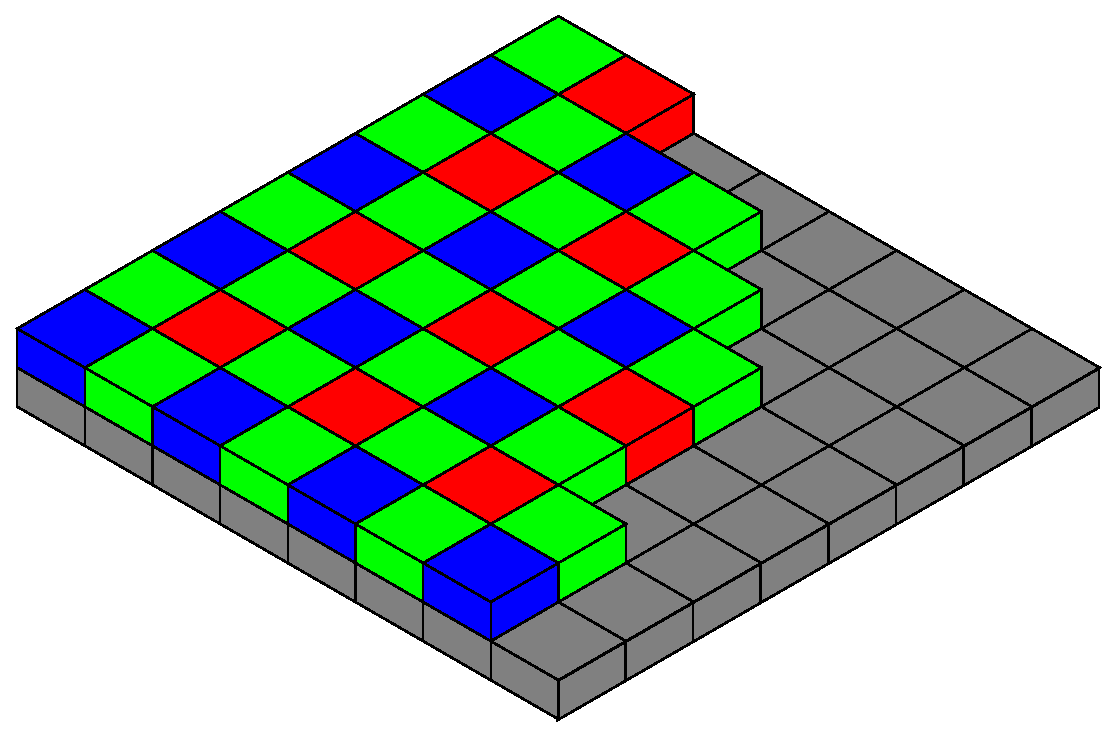
\includegraphics[width=0.6\textwidth]{BayerPattern.pdf}
	\caption{Bayer-Matrix auf einem Sensor\cite{bayerPattern06}}
	\label{fig:bayerPattern}
\end{figure}

Auf Grund der Menge an Bildern und dem damit verbundenen Speicherbedarf wurden die Bilder zunächst in das PNG-Dateiformat übertragen.
Danach müssen zunächst die gebayerten Dateien mittels eines Vorgangs, der als \textit{demosaicing} bezeichnet wird,
als Farbbilder rekonstruiert werden.
Das geschiet mit einem Skript des Frauenhofer IOSB, das die Open Source Computer Vision Library OpenCV \footnote{https://opencv.org/} benutzt.
% Dies geschieht mittels der Open Source Computer Vision Library OpenCV \footnote{https://opencv.org/}, die ein Bild von einem Farbraum in einen anderen übertragen kann.
Dieses Skript wurde angepasst und damit und dann damit die einzelnen Bilder in RGB-Farbbilder konvertiert.
% Ein Skript, das vom Fraunhofer IOSB zur Verfügung gestellt wurde, wurde angepasst und damit die einzelnen Bilder in RGB-Farbbilder konvertiert.
% \todo[inline]{Skript ursprünglich von Georg, ein paar changes implementiert (bezüglich input und output.)}
Auf diesen Bildern kann dann eine Segmentierung vorgenommen werden.
Dafür wurde ebenfalls ein existierendes Skript des Fraunhofer IOSBs angepasst, in dem erneut die Computer Vision Library OpenCV benutzt wird.
Für jede Sorte von Schüttgut wurde ein eigenes Parameterprofil von Hand optimiert.
Ein solches Parameterprofil besteht aus einem oberen und unteren Grenzwert in jedem Kanal des HSV-Raums und einer minimalen Fläche, die ein Teilchen umfassen muss.
Entsprechend der im Profil festgelegten Parameter werden für die einzelnen Bilder Masken angelegt,
die angeben ob die HSV-Werte der einzelnen Pixel innerhalb oder außerhalb der Grenzwerte liegen. 
Mit diesen Masken werden dann alle möglichen Konturen von Schüttgutpartikeln extrahiert. 
Die Konturen werden dann bezüglich der Plausibilität ihrer Größe und Form gefiltert. 
Im letzten Schritt wird nun der gewichtete Mittelpunkt der verbleibenden Konturen bestimmt und abgespeichert.


Das Ergebnis von diesem Segmentierungsskripts ist eine CSV-Datei für jeden Batch.
Ein Beispiel für einen Ausschnitt aus solch einer Datei ist in Tabelle~\ref{table:Segmentierungsscript} zu sehen.
Eine Zeile repräsentiert jeweils ein Bild aus dem Batch, also einen Zeitschritt.
Zu Beginn jeder Zeile steht zunächst die Frame-Nummer, gefolgt von der Anzahl der detektierten Partikel
und den Koordinaten der Mittelpunkte der detektierten Partikel.
Aus den Mittelpunkten in dieser CSV-Datei werden nun mittels des in \textsc{Matlab} implementierten \textit{Multi-Target-Tracking}-Algorithmus die in dem Datensatz vorhandenen Tracks abgeleitet,
% \todo{Mehr details: Tracksort trackzuweisung Assignment Problem. Referenz Tobi MA?}
die dann wiederum in einer neuen CSV-Datei gespeichert werden.
Die einzelnen Tracks werden als Spaltenpaare dargestellt, mit jeweils einer Spalte für die X- und Y-Koordinaten und einer Zeile für jeden Zeitschritt.
Ein Ausschnitt aus einer solchen Datei ist in Tabelle \ref{table:tracksortCSV} zu sehen.
Dies ist der Zustand in dem die Daten dann im Programmcode geladen werden. 

\begin{table}[p]
    \caption{Ausschnitt aus dem Ergebnis des Segmentierungsskripts}
	\small
	\centering
    \begin{tabular}{@{}rcrrrrrr@{}}
    \toprule
    Frame   & \#MP & MP\_1\_x  & MP\_1\_y  & MP\_2\_x  & MP\_2\_y  & MP\_3\_x & MP\_3\_y \\ \midrule
    636     & 1    & 1222.9975 & 92.7641   & NaN       & NaN       & NaN      & NaN      \\
    637     & 1    & 1223.4063 & 182.9758  & NaN       & NaN       & NaN      & NaN      \\
    638     & 1    & 1223.6052 & 273.2425  & NaN       & NaN       & NaN      & NaN      \\
    639     & 1    & 1223.7067 & 364.0339  & NaN       & NaN       & NaN      & NaN      \\
    640     & 1    & 1224.0704 & 453.9057  & NaN       & NaN       & NaN      & NaN      \\
    641     & 2    & 1224.2051 & 544.5191  & 1692.4549 & 43.8822   & NaN      & NaN      \\
    642     & 2    & 1224.5793 & 634.7288  & 1696.6901 & 135.9595  & NaN      & NaN      \\
    643     & 2    & 1224.9082 & 726.0094  & 1700.451  & 229.1195  & NaN      & NaN      \\
    644     & 2    & 1225.2296 & 815.9663  & 1704.1472 & 321.2075  & NaN      & NaN      \\
    645     & 2    & 1225.4286 & 906.7078  & 1708.0593 & 414.2785  & NaN      & NaN      \\
    646     & 2    & 1225.7588 & 996.0286  & 1711.5309 & 506.0545  & NaN      & NaN      \\
    647     & 3    & 1226.0411 & 1086.5729 & 1714.8831 & 599.5417  & 961.8821 & 62.7111  \\
    648     & 3    & 1226.2337 & 1175.9271 & 1718.1401 & 691.6325  & 958.5526 & 154.3124 \\
    649     & 3    & 1226.2073 & 1265.7495 & 1721.6618 & 784.5927  & 955.3107 & 246.5241 \\
    650     & 3    & 1226.2543 & 1354.9362 & 1724.9158 & 876.7192  & 952.4919 & 338.1123 \\
    651     & 3    & 1226.2634 & 1444.5903 & 1728.3341 & 970.2909  & 949.2896 & 430.9692 \\
    652     & 3    & 1226.0845 & 1533.0901 & 1732.1745 & 1062.4624 & 946.3455 & 522.8667 \\
    653     & 3    & 1225.7319 & 1621.8461 & 1735.8759 & 1155.2937 & 943.3384 & 615.4545 \\
    654     & 2    & 1739.6714 & 1247.1867 & 940.2511  & 707.7306  & NaN      & NaN      \\
    655     & 2    & 1743.4279 & 1339.4146 & 937.2216  & 800.4557  & NaN      & NaN      \\
    656     & 2    & 1747.1525 & 1430.2501 & 934.5311  & 891.7249  & NaN      & NaN      \\
    657     & 2    & 1750.9771 & 1521.8102 & 931.6626  & 984.2284  & NaN      & NaN      \\
    658     & 2    & 1754.1491 & 1612.5565 & 928.7587  & 1076.4749 & NaN      & NaN      \\
    659     & 1    & 925.8463  & 1168.794  & NaN       & NaN       & NaN      & NaN      \\
    660     & 1    & 922.8752  & 1260.7461 & NaN       & NaN       & NaN      & NaN      \\
    661     & 1    & 920.2056  & 1352.8549 & NaN       & NaN       & NaN      & NaN      \\
    662     & 1    & 917.4051  & 1444.3431 & NaN       & NaN       & NaN      & NaN      \\
    663     & 1    & 914.6493  & 1535.5131 & NaN       & NaN       & NaN      & NaN      \\
    664     & 1    & 911.8565  & 1626.5341 & NaN       & NaN       & NaN      & NaN      \\ \bottomrule
    \end{tabular}
    \normalsize
    
    \label{table:Segmentierungsscript}
    \end{table}


\begin{table}[p]
	\caption{Ausschnitt aus dem Ergebnis des \textit{Multi-Target-Tracking}-Algorithmus}
	\label{table:tracksortCSV}
    \small
    \centering
    \begin{tabular}{@{}rrrrrr@{}}
    \toprule
    TrackID\_4\_X & TrackID\_4\_Y & TrackID\_5\_X & TrackID\_5\_Y & TrackID\_6\_X & TrackID\_6\_Y \\ \midrule
    1036.4613     & 82.3719       & 1899.9239     & 83.2049       & 1654.4423     & 50.6811       \\
    1033.0189     & 174.9809      & 1896.8142     & 171.3283      & 1655.3193     & 143.9749      \\
    1029.6167     & 266.4979      & 1893.5937     & 259.8098      & 1656.0221     & 237.1573      \\
    1026.3908     & 358.4831      & 1890.3912     & 348.1731      & 1656.8966     & 329.8636      \\
    1023.0203     & 449.6429      & 1887.1035     & 436.4588      & 1657.6308     & 423.1592      \\
    1019.5391     & 542.2334      & 1883.7761     & 525.1073      & NaN           & NaN           \\
    NaN           & NaN           & 1880.2716     & 613.0896      & NaN           & NaN           \\
    NaN           & NaN           & 1876.6054     & 701.9719      & NaN           & NaN           \\
    NaN           & NaN           & NaN           & NaN           & NaN           & NaN           \\ \bottomrule
    \end{tabular}
\end{table}






\section{Simulierte Daten}

% \color{blue}
% Die DEM Daten, wo sie herkommen, was der unterschied ist zu den selbst aufgenommenen Daten. 
% Vorteile und Nachteile...\cite{pieper2016numerical}, \cite{pieper2017numerical} 

% Original: \SI{1000}{\hertz}, downsampled auf \SI{200}{\hertz}, 

% Nicht ganz so viele Partikel, aber dafür sehr lange tracks - Informationen auf dem gesamten Band, nicht nur auf dem Part wo die Kamera drauf schaut.

% Vergleich bezüglich der Eignung für die verschiedenen Ansätze dann im Evaluations Kapitel
% \color{black}

Neben den selbst aufgenommenen Daten wurde im Rahmen dieser Arbeit auch mit einigen existierenden Datensätzen gearbeitet.
Diese Datensätze wurden basierend auf einer hochgenauen numerischen Simulation des \textit{TableSort} Systems mittels der Diskrete-Elemente-Methode erstellt~\cite{pieper2016numerical}\,\cite{pieper2017numerical}.
% \todo{interaktion Teilchen untereinander und mit dem Sortierer?}
In Abbildung~\ref{fig:DEMSimulation} ist die virtuelle Nachbildung des Schüttgutsortierers zu sehen, auf dem die Simulation durchgeführt wurde.
% Die Simulation wird mit einem Zeitschritt von \SI{1e-5}{\second} durchgeführt.
Die Positionsdaten in den Datensätzen waren ursprünglich mit einer Frequenz von \SI{1000}{\hertz} aufgelistet.
Um jedoch Vergleichbarkeit mit den realen Daten zu erhalten wurde diese Frequenz auf \SI{200}{\hertz} reduziert.
Die Positionsangaben der Simulation werden in Metern angeben.
Das Förderband erstreckt sich entlang der y-Achse von \SI{0.0}{\meter} bis \SI{0.18}{\meter} und entlang der x-Achse von \SI{0.388}{\meter} bis \SI{0.788}{\meter} 

Dennoch gibt es einige Unterschiede zwischen den selbst aufgenommenen und den simulierten Daten.
Von diesen Unterschieden ist der schwerwiegendste, dass die Positionen der simulierten Partikel eine absolut verlässliche Ground~Truth sind, 
die direkt aus Simulation entnommen wurde.
So verlässlich sind die Partikelpositionen bei den selbst aufgenommen Daten nicht.
Während den einzelnen in Sektion~\ref{sec:pipeline} beschrieben Schritten kann es zu Fehlern kommen, die sich durch die gesamte Pipeline fortpflanzen.
Die Segmentierung kann an einigen Stellen nicht präzise sein, indem z.\,B. ein Stück Schattens als Teil des Partikels interpretiert wird und dadurch den Mittelpunkt verschiebt. 
Bei einer Kollision von zwei Partikeln kann es dazu kommen, dass der \textit{Multi-Target-Tracking}-Algorithmus die beiden Tracks vertauscht.  
Des Weiteren bewegt sich das Förderband in der Simulation mit \SI{1.5}{\meter\per\second}, 
während Messungen am realen \textit{TableSort} System darauf hindeuten, dass das Förderband dort nur eine Geschwindigkeit von 
circa \SI{1.1}{\meter\per\second} hat.
Ein weiterer Unterschied ist der Aufnahmebereich.
Im Gegensatz zu den selbst aufgenommenen Daten, die nur Informationen 
zu den Bewegungen der Partikel im Bereich auf den die Hochgeschwindigkeitskamera gerichtet ist umfassen, 
befinden sich in den DEM Datensätzen die Positionen der Teilchen über die gesamte Länge des Förderbandes.
Das bedeutet auch, dass in den DEM Datensätzen die Phase der Partikel bevor und während sie vom Förderband beruhigt werden enthalten ist.
Außerdem hat es zur Folge, dass die individuellen Tracks deutlich länger sind, sprich mehr Messungen enthalten.
Bei der NextStep Prädiktion sorgt das dafür, dass es eine deutlich größere Anzahl an Feature-Label-Paaren gibt.
Die Bewegungsrichtung der Partikel ist ebenfalls nicht identisch.
Während die selbst aufgenommenen Datensätze eine Bewegung entlang der y-Achse haben, bewegen sich die simulierten Partikel entlang der x-Achse.
% \todo[inline]{Einheit real: Pixel, Einheit simuliert: m}
\todo[inline]{simulierte haben viel mehr Partikel gleichzeitig auf dem Band - mehr kollisionen...?}

\begin{figure}[h]
    \centering
    % \missingfigure{DEM Simulationsgrafik}
	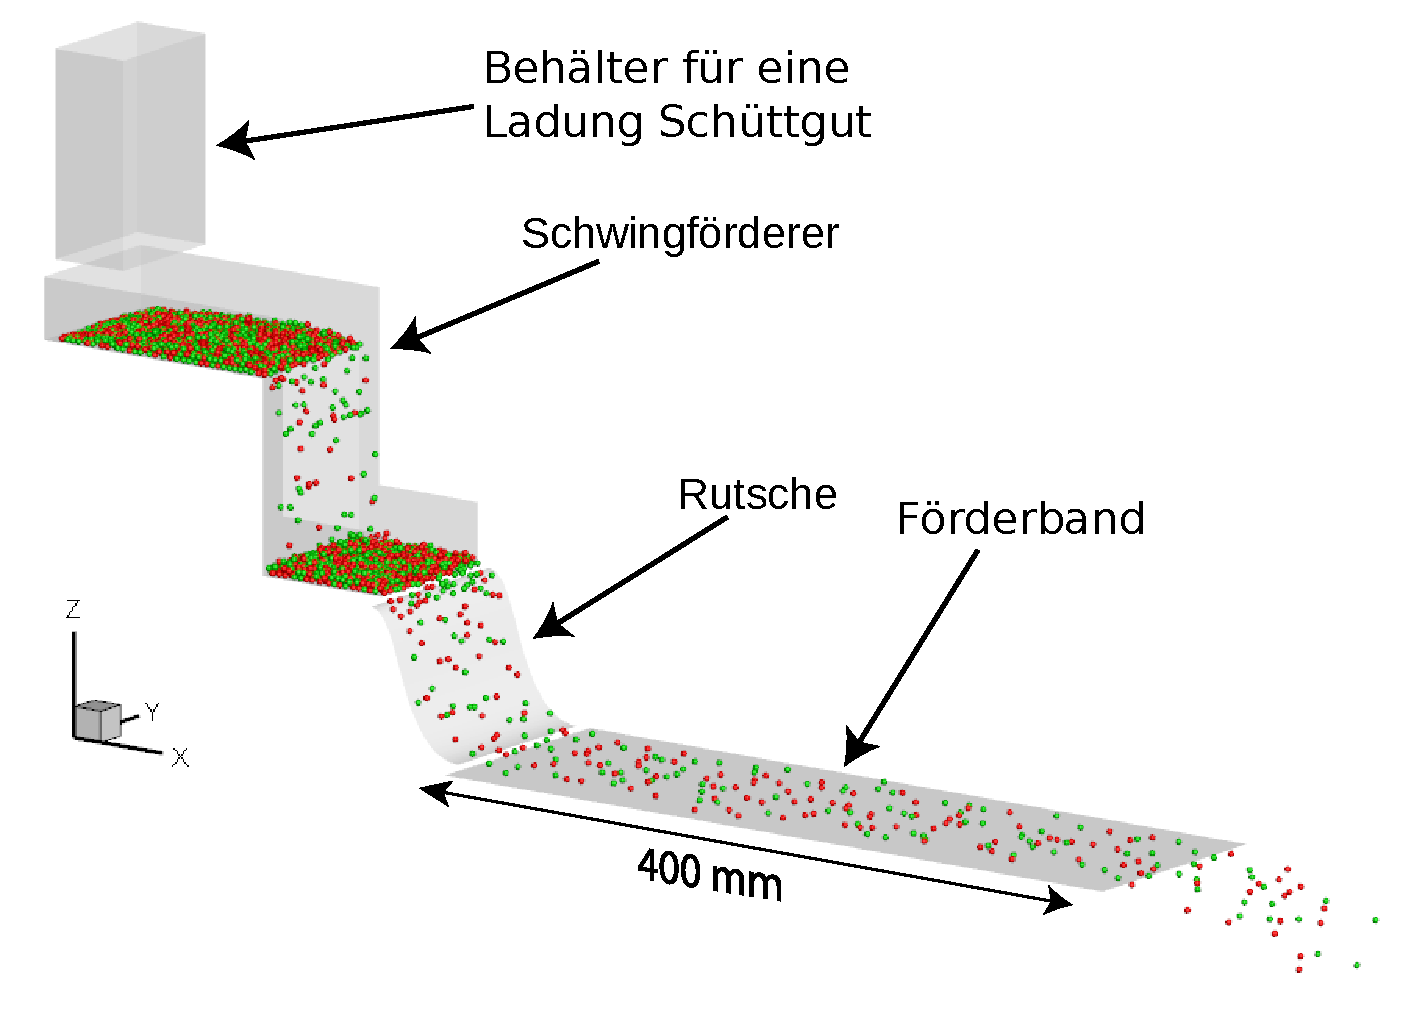
\includegraphics[width=\textwidth]{DEM-SimOverview}
	\caption{Visualisierung der DEM Simulation, übersetzt~aus~\cite{Pfaff2018}}
	\label{fig:DEMSimulation}
\end{figure}



\section{Datenformatierung}

% \color{blue}
% \begin{itemize}
% 	\item Zu Beginn des Datenverarbeitungskapitel erstmal definieren wie unsere Feature-Label-Paare aussehen.
% 	\item Features eigentlich immer gleich:
% 	\item die Positionen der letzten \(n\) Zeitschritte (FeatureSize Hyperparameter)
% 	\item also ein \(2n\) Tupel, mit jeweils \(n\) X-Koordinaten und \(n\) Y-Koordinaten
% 	% \item \(n\) \textit{n} \(n\) \(n\) \textit{n}
% \end{itemize}

% Labels: Unterscheidung nach Anwendung:

% NextStep: Label ist 2-Tupel, X und Y Koordinate
% Separator: 
% 	gegeben ist eine Stelle entlang der Bewegungsrichtung der Teilchen an der der Separator angebracht ist.
% 	erstes element des Label ist die Koordinate entlang der orthogonalen Achse zur Bewegungsrichtung wo das Teilchen den Separator passiert
% 	zweites Element ist die Anzahl von Zeitschritten , die das Teilchen noch bis zum Separator braucht.

% Important Point: Labels wurden normalisiert und Standardisiert ( \(\frac{TrueVal - Mean}{Standard Diviation}\))
% um auszugleichen, dass sich Position und Zeitschritte auf unterschiedlichen Skalen bewegen und dementsprechend unterschiedlich hohe gradienten haben.


% Es ist implementiert, dass die verschiedenen Dimensionen unterschiedlich stark gewichtet werden können - Je nach Schüttgut/präzision des Separators
% Aber für die evaluierung ist keine Gewichtung vorgenommen worden.

% optional: Histogramme über die Daten (mehr Teilchen in der Mitte bei Location...)
% \color{black}

Das Format, das die Daten annehmen, ist für die NextStep- und den Separator Netze leicht unterschiedlich.
%  unterscheidet sich leicht zwischen den beiden Anwendungen.
Die Feature-Label-Paare der unterschiedlichen Anwendungen unterscheiden sich nur in den Labeln.
Die Eingangsdaten sind -- abhängig von einem Hyperparameter --
in beiden Fällen die Position des Partikels zu den letzten \(n\) Zeitschritten.
Deshalb muss beim Format der Features kein Unterschied zwischen der Art der Aufgabe gemacht werden.
Dieser Hyperparameter wird \textit{FeatureSize} genannt. 
Die Features sind also ein \(2n\)-Tupel, bestehend aus \(n\) X-Koordinaten und \(n\) Y-Koordinaten 
von den Mittelpunkten der \(n\) beobachteten Teilchen.
Die Reihenfolge der Features ist für das neuronale Netz irrelevant, solange sie konsistent zwischen Training und Evaluation bleibt.
Was die Reihenfolge der Features angeht, so ist sie für das neuronale Netz irrelevant, 
solange sie konsistent zwischen Training und Evaluation bleibt. 
In der umgesetzten Implementierung ist es so, dass zuerst die X-Koordinaten 
und dann die Y-Koordinaten in chronologischer Reihenfolge aufgereiht sind. 



Die Labels, die das NextStep-Netz benutzt, sind \(2\)-Tupel.
Diese bestehen aus den X- und Y-Koordinaten des Partikels im nächsten Zeitschritt.
Wie in Abbildung~\ref{fig:FLPNext} dargestellt, befinden diese sich in der nächsten Zeile nach den Features.
% Es handelt sich um die X- und Y-Koordinate der Position des Partikels im nächsten Zeitschritt.
% Diese findet man als die nächste Zeile des Doppelspalte des dazugehörigen Tracks.
% \todo{Grafik um es verständlicher zu machen? Siehe zwischevortrag}

\begin{figure}
	\centering
	% \missingfigure{geometrische Bestimmung des Schnittpunkts mit dem Separator}
	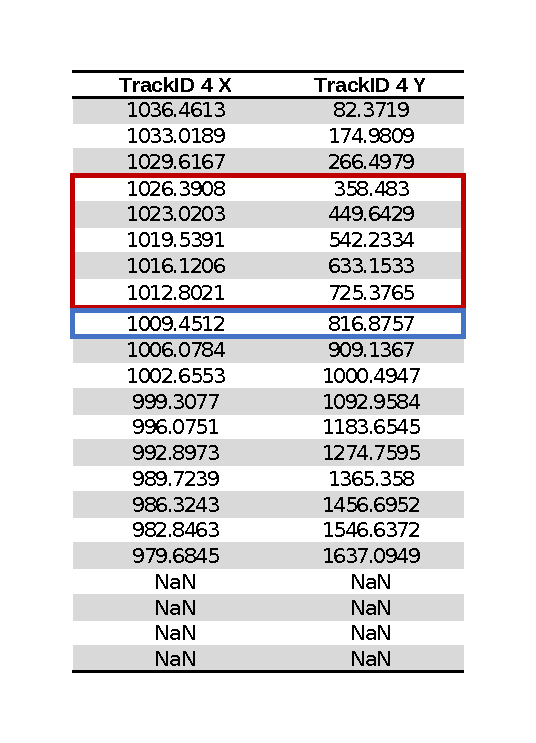
\includegraphics[width=0.6\textwidth]{weizen_003_trackHistory_NothingDeleted-v3}
	\caption[Beispiel Feature-Label-Paar NextStep]{An diesem Ausschnitt eines Tracks wird beispielhaft mit FeatureSize 5 gezeigt, wie die einzelnen Feature-Label-Paare im NextStep Fall entstehen.
		Der rote Rahmen markiert die 10 Features. Der blaue Rahmen markiert das dazugehörigen Label. 
		% Der blaue und der rote Rahmen werden parallel entlang des Tracks verschoben um alle möglichen Feature-Label-Paare zu erhalten. 
		}
	\label{fig:FLPNext}
\end{figure}


Die Labels des Separator-Netzes sind ebenfalls \(2\)-Tupel.
Im Gegensatz zu denen des NextStep-Netzes können diese nicht direkt aus der CSV-Datei ausgelesen werden, da sie nicht gemessen werden.
Stattdessen müssen sie berechnet werden.
Dies ist in Abbildung~\ref{fig:Schnittpunkt} dargestellt.
Für jedes Partikel müssen die letzte Position vor dem Überqueren des Druckluftdüsenarrays \(f_n\) 
und die erste Position nach dem Überqueren \(f_{n+1}\) bestimmt werden.
In Abbildung~\ref{fig:FLPSep} sind dies die blau markierten Einträge. 
Dabei wird die angenommen, dass die Geschwindigkeit des Partikels zwischen \(f_n\) und \(f_{n+1}\) konstant ist.
Dies ist eine Approximation, die ebenfalls in~\cite{Pfaff2018} verwendet wird.
Das erste Element eines jeden Labels ist die Koordinate entlang der Achse orthogonal zur Bewegungsrichtung des Förderbandes, wo das Partikel den Druckluftdüsenarray passiert.
\todo{Bewegungsrichtung Band in der Grafik klarer machen}
Diese erhalten wir, indem wir den Schnittpunkt \(s\) zwischen der Strecke \(f_n\) nach \(f_{n+1}\) und 
der Gerade des Druckluftdüsenarray bestimmen.
Das zweite Element ist die Zeit, die das Partikel noch brauchen wird, bis es das Druckluftdüsenarray passiert.
Sie wird in der Einheit Frames angegeben.
Die ganzzahlige Komponente hiervon ist durch das Zählen der Messungen im Track zu bestimmen.
Die Nachkommastelle wird bestimmt als das Verhältnis von der Distanz zwischen \(f_n\) und \(s\), 
und der Distanz zwischen \(f_n\) und \(f_{n+1}\).
% \todo[inline]{Example: Gegeben ein Track, was für Features und Labels würden da rausfallen}

\begin{figure}[h]
	\centering
	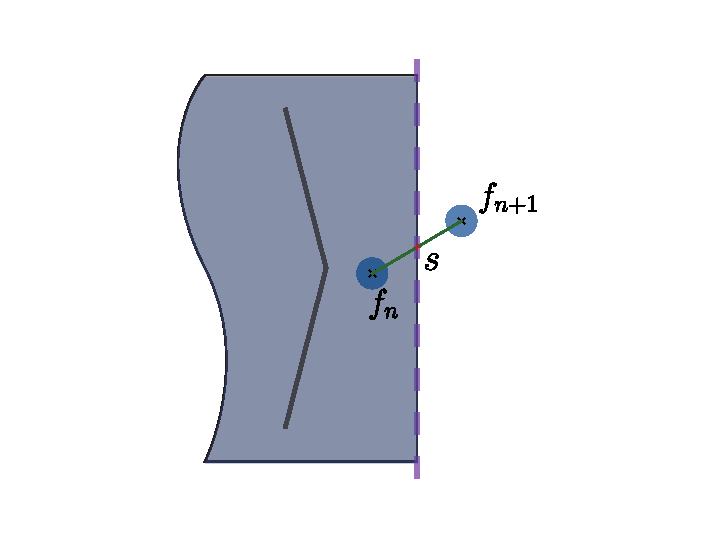
\includegraphics[width=\textwidth]{geometrie}
	\caption{Geometrische Bestimmung der Labels, nach \cite{Pfaff2018}}
	% \todo{Quelle - test?}
	\label{fig:Schnittpunkt}
\end{figure}

\begin{figure}[h]
	\centering
	% \missingfigure{geometrische Bestimmung des Schnittpunkts mit dem Separator}
	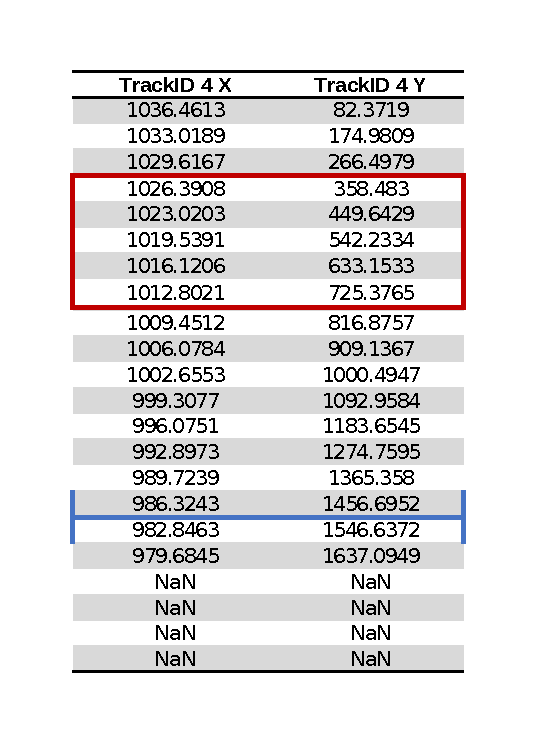
\includegraphics[width=0.6\textwidth]{weizen_003_trackHistory_NothingDeleted_sep-v3}
	\caption[Beispiel Feature-Label-Paar Separator]{An diesem Ausschnitt eines Tracks wird beispielhaft mit FeatureSize 5 gezeigt, wie die einzelnen Feature-Label-Paare im Separator Fall entstehen.
	Analog zu Abbildung~\ref{fig:FLPNext} ist ein Featurevektor markiert. Der Unterschied besteht in der Bestimmung der Labels. 
	Der Schnittpunkt mit dem Druckluftdüsenarray befindet sich zwischen den beiden blau markierten Messungen und kann dementsprechend nicht direkt abgelesen werden.}
	% \todo{Quelle - test?}
	\label{fig:FLPSep}
\end{figure}


% Um zu verhindern, dass verschiedene Label-Elemente basierend auf ihrer Skalierung beim Training unterschiedlich stark gewichtet werden, werden sie standardisiert.
Damit die Fehler der beiden Labelelemente sich ähnlich auf den Gesamtgradienten auswirken,
selbst wenn ihre Werte in sehr unterschiedliche Wertebereichen liegen oder einfach unterschiedliche Einheiten haben, werden die Labels komponentenweise standardisiert.
Dieses Problem würde zum Beispiel auftreten, wenn sich die Werte des einen Elements im Bereich zwischen 0 und 1700 bewegen, während die des Anderen zwischen 1 und 25 liegen,
so wie es bei den Separator Netzen der Fall sein kann.
Bei dem NextStep Fall wäre die Standardisierung nicht zwingend notwendig, 
sie wurde allerdings, um die Einheitlichkeit zu wahren, für beide Fälle implementiert. 
Für die Standardisierung wird von der jeweiligen Komponente der Mittelwert und die Standardabweichung berechnet. 
Im Anschluss wird vom jeweiligen Eintrag \(X\) der zugehörige Mittelwert \(\mu\) subtrahiert, und durch die korrespondierende Standardabweichung \(\sigma\) dividiert
% Jedes Labelelement \(e\), sei es das erste oder das zweite Element seines entsprechenden Tupels, wird gemäß seiner Position vor dem Training angepasst,
% indem davon der Durchschnitt aller ersten beziehungsweise zweiten Elemente abgezogen wird und dann durch die Standardabweichung aller ersten beziehungsweise zweiten Elemente geteilt wird.
\todo[inline]{ist das hier verständlich?}
	
\begin{equation*}
	X_{\text{neu}} = \frac{X - \mu}{\sigma} %\mu_{\text{N}}}{\sigma_{\text{N}}}
\end{equation*}

Durch die Standardisierung wird jedes Label so skaliert, dass die beiden Elemente der Labels jeweils einen Erwartungswert von 0.0 und eine Standardabweichung von 1.0 haben.
Die Ausgaben des Netzes müssen umkehrt zurück in das ursprüngliche Format umgerechnet werden.
% \todo{überlegen wie ich klar mache, dass es sich um den durchschnitt und die Abweichung der jeweiligen Spalte handelt}

% \todo[inline]{Der Absatz hier nach Implementierung verschieben?}
Im Code gibt es die Möglichkeit, unterschiedliche Label-Elemente unterschiedlich zu gewichten, indem Weighted Mean Squared Error als Fehlerfunktion verwendet werden kann. 
Von dieser Möglichkeit wird in den später vorgestellten Ergebnissen nicht Gebrauch gemacht, beziehungsweise den beiden Elementen wird jeweils das Gewicht~1.0 zugewiesen.
Diese Option könnte nützlich sein, falls die Ansteuerung der Druckluftdüsen eine maximale Auflösung hat, jenseits derer eine bessere Zeitprädiktion keine Verbesserung der Sortierqualität mehr erzielt.
% \todo{hier noch schreiben, warum man das tun wollen könnte, oder nicht?}





% Menge in gecleanten Daten:

% 7343 Kugeln
% 6824 Pfefferkörner
% 15760 Zylinder
% 8426 Weizenkörner


\section{Datenaugmentierung}

% \color{blue}

% Cleanup : FilterTracksByAngle, FilterByVectorLengthChange \todo{Überlegen ob ich da so viel aufschreiben soll - 
% minimaler unterschied nach Resegment (Bessere Tracksort zuordnung?)}

% \begin{itemize}
% 	\item Data Augmentation: Definition und Beschreibung
% 	\item bei Bildern normalerweise Rotieren, Translation, Ausschnitte...
% 	\item Hier: Spiegeln
% 	\item in einem Band - an der Mitte, nicht die Ränder mit nehmen - Kamera nicht perfekt zentriert
% 	\item Band zentrierung filter
% 	\item führt zu: Beinah Verdoppelung der Feature-Label-paare fürs training.
% \end{itemize}
% \color{black}

Als Datenaugmentierung oder auch Data Augmentation bezeichnet man Verfahren, die dem eigenen Datenset Datenpunkte hinzufügen ohne zusätzliche Daten aufzunehmen.
Man generiert aus den bestehenden Daten zusätzliche, synthetische Daten, die dann im Trainingsset eingesetzt werden können.
Ausreichend viele Trainingsbeispiele zu haben ist notwendig, um mit neuronalen Netzen eine gute Performance zu erzielen.
Die synthetischen Beispiele müssen jedoch konsistent mit den Originaldaten sein, da sie sonst die Qualität der Ausgabe des Netzes negativ beeinträchtigen können.

Für Netze, die in der Computer Vision eingesetzt werden gibt es einige weit verbreitete Techniken,
zum Beispiel Rotation, Translation, Spiegeln und das Ausschneiden von Teilbildern.

Für den gegebenen Fall mit den Mittelpunkten von Schüttgut-Partikeln als Features resultiert von diesen Techniken nur das Spiegeln in sinnvollen Daten.
Eine beispielhafte Darstellung der vorgenommenen Data Augmentation ist in Abbildung~\ref{fig:dataAugm} zu finden.
Gespiegelt wird an der Mittellinie des Bands, beziehungsweise der Rutsche entlang der Bewegungsrichtung.
Tracks, die eine gewisse Distanz zur Spiegelachse überschreiten, werden ausgenommen, da zumindest bei den selbst aufgenommenen Daten 
die Kamera nicht perfekt zentriert ist.
Deshalb könnte nicht ausgeschlossen werden, 
dass unrealistische Feature-Label-Paare dem Trainingsset hinzugefügt werden würden.

Die Anwendung dieser Technik auf die vorhandenen Daten führt beinahe zu einer Verdoppelung 
der benutzbaren Feature-Label-Paare im Trainingsset, wovon man sich einen positiven Effekt auf die Qualität der Ergebnisse verspricht.

\begin{figure}[h]
	% \missingfigure{Visualisierung Dataaugmentation}
	\centering
	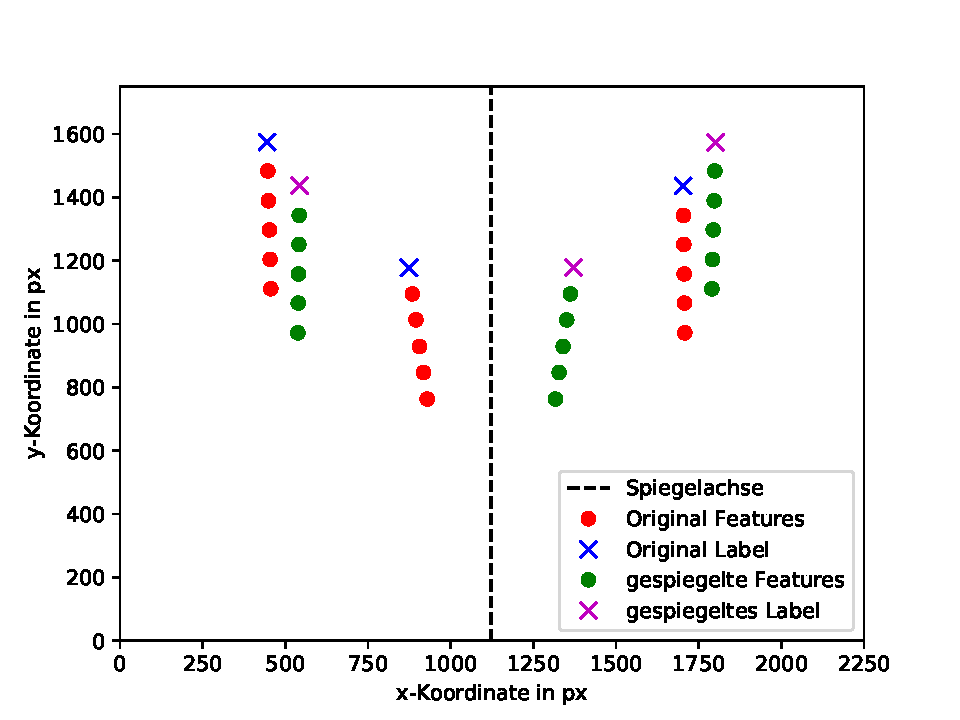
\includegraphics[width=\textwidth]{augmentationImage.pdf}
	\caption{Visualisierung der Datenaugmentierung durch Spiegelung}
	% \todo{Quelle Bild!}
	\label{fig:dataAugm}
\end{figure}



\section{Datenumfang}

Im Rahmen dieser Arbeit wurden insgesamt 247\,951 Bilder aufgenommen.
Davon waren 177\,951 Bilder auf dem Förderband und 70\,000 Bilder auf der Rutsche.
Die Verteilung dieser Bilder ist in Abbildung~\ref{fig:barPics} dargestellt.

\begin{figure}[h]
	% \missingfigure{Visualisierung Dataaugmentation}
	\centering
	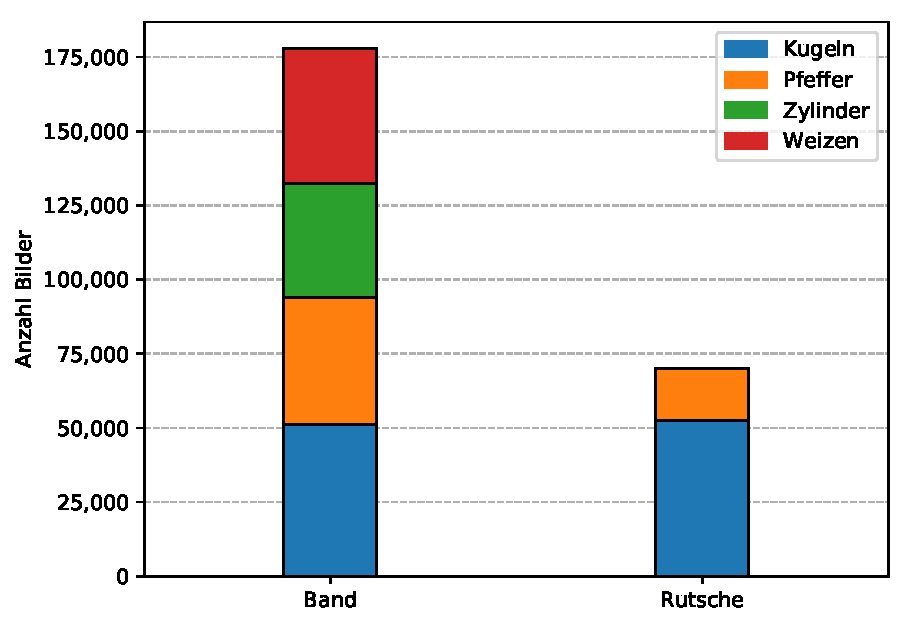
\includegraphics[width=\textwidth]{ImagesAmountPictures}
	\caption{Balkendiagramm Verteilung Bilder}
	% \todo{Quelle Bild!}
	\label{fig:barPics}
\end{figure}

Der \textit{Multi-Target-Tracking}-Algorithmus wurde benutzt um die Anzahl der Kugeln zu bestimmen.
Auf dem Förderband wurden 7712 Tracks von Kugeln,
7170 Tracks Pfefferkörnern,
19\,200 Tracks von Zylindern,
und 8702 Tracks von Weizenkörner zugeordnet.
Zudem wurden 5132 Tracks Kugeln und 3609 Tracks von Pfefferkörner auf der Rutsche zugeordnet.

Im DEM Datensatz sind die Tracks von 3713 Kugeln, 4357 Plättchen und 4427 Zylindern enthalten.
Die Verteilung der Tracks ist in Abbildung~\ref{fig:barTracks} zu sehen.

\begin{figure}[h]
	% \missingfigure{Visualisierung Dataaugmentation}
	\centering
	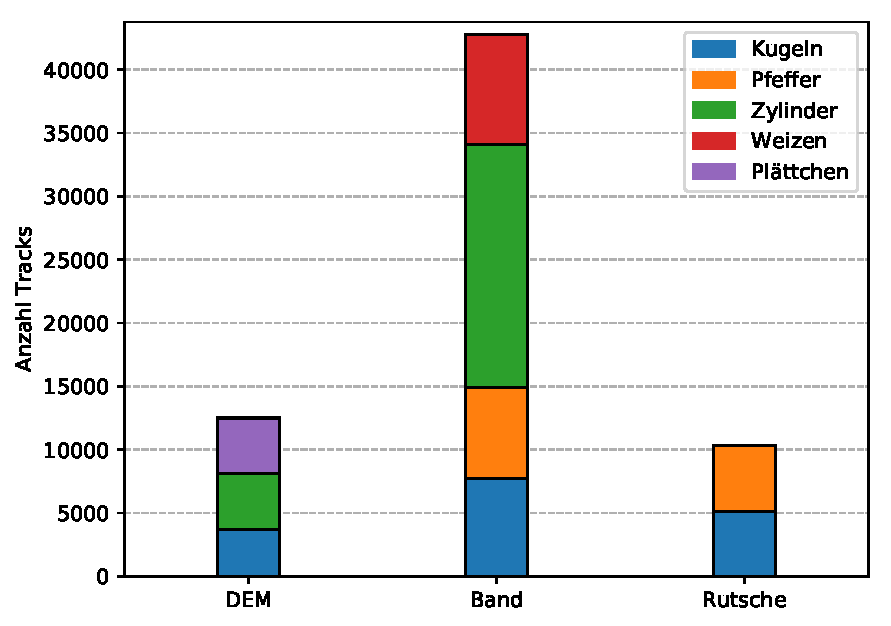
\includegraphics[width=\textwidth]{ImagesAmountTracks}
	\caption{Balkendiagramm Verteilung Tracks}
	% \todo{Quelle Bild!}
	\label{fig:barTracks}
\end{figure}

Die Feature-Label-Paare, die aus den Tracks extrahiert werden, 
müssen in ein Trainingsset und ein Testset aufgeteilt werden.
In manchen Situationen wird noch ein drittes Set, das so genannte Validationset, benötigt.
Dies ist zum Beispiel beim Hyperparameter Tuning der Fall.

Hierbei ist wichtig, dass das Testset eine gute Repräsentation des gesamten Datensets ist 
und ausreichend groß ist um statistisch aussagekräftige Ergebnisse zu produzieren.
Im Rahmen dieser Arbeit wurde meist eine Aufteilung im Verhältnis 90:10 zwischen Trainings- und Testset vorgenommen.
Es ist jedoch möglich beliebige andere Splits in der Hyperparameter Datei festzulegen.
% \todo{Vorgriff zum nächsten Kapitel - hier wissen wir noch gar nicht, dass ich ein Hyperparameter File habe...}  




% Train - Test - Validation - Split:
% Train - test, 90\% zu 10\%.
% Validation nur für die sets auf denen das Hyperparameter Tuning gemacht wurde
% [ungefähres ]

% \todo[inline]{Table mit Anzahl von Elementen in verschiedenen Batches?}

% \begin{figure}[h]
%     \centering
%     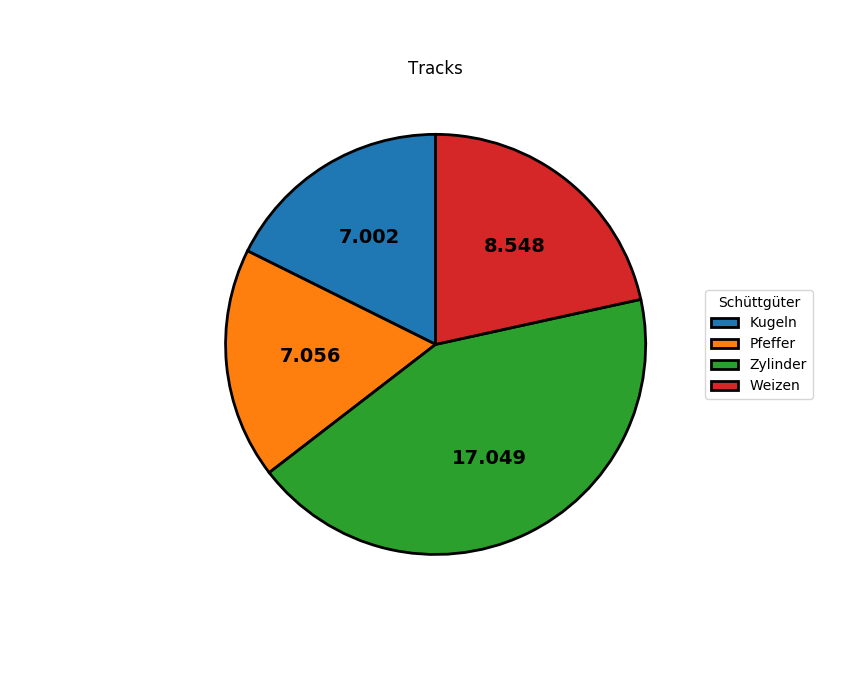
\includegraphics[width=\textwidth]{img/scaledPieChart-trimmed}
%     \caption{Verteilung Schüttgut Elemente nach Sorte}
%     \label{piechartSchuettgut}
% \end{figure}



% Features:
% NextStep einfach alle \(n\)--Tupel, die ein Track hergibt, sodass es noch ein Label geben würde
% Separator: Muss unterschieden werden - Filtern oder nicht filtern, danach ob es das letzte mögliche Tupel vor der prediction Phase ist.
% Mit filtern besseres ergebnis, aber auch deutlich weniger Trainingsbeispiele (Overfitting wird mehr zur Gefahr)
% Ohne Filtern: Flexibler und mehr Trainingsbeispiele - man könnte im Nachhinen den PredictionCutOff verlegen 
% und einfach das Netz weiter verwenden ohne neu zu trainieren.
% Maybe ein Mittelding, das man nicht alle tupel nimmt aber auch nicht nur die letzten? Ausblick, zukunft



% Labels:
% Sehr straight forward für NextStep (Literally), einfach die nächste Zeile im Track jeweils für X und Y

% für separator slightly more complicated: 
% Element des Tracks vor und hinter der Separator position (entlang der Travel Achse)

% Schnittpunkt geometrisch bestimmen.
% Label für position ist die Position entlang der Achse orthogonal zur Bewegungsrichtung vom Schnittpunkt der Separatorlinie und 
% der Strecke zwischen dem Element vor und dem element hinter. siehe \ref{fig:Schnittpunkt}




% \todo{table of size of different data sets - number of pictures...}

% \color{blue}
% Verhältnis: Anzahl Feature-Label-Paare für verschiedene Beispiele und verschiedene Settings
% (FeatureSize, Filter Ja/Nein, Augmentation Ja/Nein) Als Tabelle?

% OUTDATED:
% Bei einer FeatureSize von 5 ergeben sich bei den Kugeln so 98.966 Feature-Label-Paare.
% Die Pfefferkörner haben dann 105.101 Feature-Le,
% bei den Zylindern kommt man auf 244.422 Feature-Label-Paare
% und bei den Weizenkörner 132.140 Feature-Label-Paare.
% \color{black}

    \chapter{Umsetzung und Implementierung}

\section{Software}

requirements.txt kann im Anhang gefunden werden mit der vollständigen Liste.

Virtual Python environment.
Implementiert in Tensorflow. (angefangen in version 1.8, später nach 1.11 upgedatet)
Datenhandling: mit Pandas. Da Data Science ein wichtiger Part der Arbeit war, sehr wichtig
erwähnen:
Matplotlib für Visualisierung (die meisten selbstgemachten grafiken hier in der Arbeit)
OpenCV für Bilderdinge in der Pipeline (wie oben erwähnt)
MATLAB, für Tracksort und die Ursprünglichen implementation der Vergleichsdinge für evaluationen 




\section{Code Struktur}


\section{Hyperparameter}

\begin{lstlisting}[language=json,firstnumber=1, caption={Beispiel eines Hyperparameter Files in JSON}, captionpos=b, label=lst-hyperparam]
    {
        "arch": {
            "dropout_rate": 0.0,
            "hidden_layers": [16, 16, 16],
            "feature_size": 5,
            "activation": "leaky_relu"
        },
        "problem": {
            "data_path": "/home/hornberger/MasterarbeitTobias/data/simulated/SpheresDownsampled",
            "modelBasePath": "/home/hornberger/MasterarbeitTobias/models/simulated/",
            "imagePath": "/home/hornberger/MasterarbeitTobias/images/",
            "separator": 0,
            "separatorPosition": 1550,
            "thresholdPoint": 1200,
            "predictionCutOff": 1300

        },
        "train": {
            "batch_size": 1000,
            "epochs": 500,
            "steps_per_epoch": 200,
            "learning_rate": 0.01,
            "optimizer": "Adam"
        },
        "data": {
            "numberFakeLines": 500,
            "testSize": 0.1,
            "augmentMidpoint": 1123,
            "augmentRange": 1000,
            "direction": "x",
            "unitLoc": "px",
            "unitTime": "1/100 Frames",    
            "limits": [0.388, 0.788, 0.0, 0.18]
        }
    }

    
\end{lstlisting}
    

\todo{Example Hyperparameter File}

\begin{itemize}
\item Architektur:
    \begin{itemize}
        \item Dropout (wird eigentlich nicht benutzt weil es regression kaputt macht), relikt vergangener Zeiten
        \item Hidden Layer: ein Array an Zahlen repräsentiert die Architektur der Hidden Layers. Jede Zahl ist ein FC Layer mit so vielen neuronen
        \item FeatureSize: Wie viele Positionen bekommt das Netz als Input ( => Größe des Inputlayers = 2x FeatureSize)
        \item Activation: Aktivierungsfunktionen für die neuronen der Hidden Layers
        % - optionen: "relu", "leaky_relu", "linear"
    \end{itemize}
\item Problem:
    \begin{itemize}
        \item DataPath: wo liegen die CSV Dateien zum die Daten rausladen
        \item ModelPath: wo soll das Netz hingespeichert werden/Hergeladen - mit Checkpoints usw.
        \item ImagePath: wo sollen Bilder hingespeichert werden, z.B. von Plot
        \item separator: 0 oder 1, jenachdem ob es den nächsten Schritt (0) oder zum Düsenbalken (1) prädizieren soll
    \end{itemize}

    Falls Separator 1:
    \begin{itemize}
        \item separationPosition: Koordinate des Düsenbalken und Ziel der Prädiktion
        \item ThresholdCutoff \todo{verify}
        \item predictionCutOff: Koordinate hinter der keine FeatureTupel mehr genommen werden
    \end{itemize}
\item Train:

\end{itemize}


\subsection{Hyperparameter Tuning}

Als Hyperparameter Optimierung oder auch Hyperparameter Tuning bezeicht man den Vorgang das am besten geeignete Set an 
Hyperparametern für einen Lernalgorithmus zu wählen.


Vorgehen bei dieser Arbeit: Jeweils für NextStep und für Separator getrennte Konfigurationen finden.

Suchen auf Simulierten Daten, weil da mehr Trainingbeispiele sind und Ergebnis auf realen Daten verifizieren.



Aktueller Stand:
NextStep: kein Overfitting gefunden => L1 und L2 Regularisierung haben keinen positiven Effekt
Adam Optimizer ist am besten
leaky_relu reigns supreme
Learning Rate Decay ist eine gute Idee. (Höherer Wert => langsamerer Zerfall)

Separator: TODO

\subsection{Architektur des neuronalen Netzes}

Input layer: \(2 * FeatureSize\) Neuronen

\(N\) hiddenlayer (as determined by Hyperparameter tuning) mit jeweils \(m\) Neuronen.
Fully connected!

Output layer:
Linear activation weil regression.
2 Neuronen, eins für die eine Label Dimension und eins für die andere.

\begin{figure}
	\missingfigure{Grafik architektur}
	% \includegraphics[width=\textwidth]{TrackSortPic}
	\caption{Architektur NN NextStep [TODO Quelle]}
	% \todo{Quelle Bild!}
	\label{fig:netArchitecture}
\end{figure}

    \chapter{Evaluation}
\label{cap:Eval}

Im vorhergegangenen Kapitel wurde die Implementierung der neuronalen Netze beschrieben.
Nun wird in diesem Kapitel betrachtet, wie gut die Ergebnisse sind, die von diesen Netzen geliefert werden.
Dazu wird zunächst beschrieben auf was für einem System das Training und die Evaluation durchgeführt wurde.
Es werden mehrere, bereits aus dem Stand der Technik bekannte Modelle beschrieben, die dann mit den Ergebnissen der neuronalen Netze 
verglichen werden.
Anschließend werden diese Ergebnisse diskutiert.
% \todo[inline]{Im vorhergegangenen Kapitel wurde beschrieben, [wie die Netze designed wurde]
% Jetzt bewerten wie gut sie das eigentlich mache.}

\section{System}

Alle in dieser Arbeit vorgestellten Netze wurden auf einem Ubuntu 18.04 Linux System trainiert und evaluiert.
Dieses verfügt über einen Intel i7-7700k CPU @ \SI{4.20}{\giga\hertz}, eine NVIDIA GeForce 1080Ti Grafikkarte mit \SI{11}{\giga\byte}~GDDR5X,
und \SI{32}{\giga\byte}~RAM. 

\todo[inline]{muss da noch irgendwie mehr dazu?}

\section{Vergleichsmodelle}

\color{blue}
Notation und Definition bei allen diesen Modellen nach Florian's Diss \cite{Pfaff2018}, mit Ausnahme von Average Acceleration.
Sei \(x(t)\) die Position des Partikels entlang der Bewegungsrichtung in Abhängigkeit von der Zeit
(continuous-time equation).
Sei \( y(t)\) die Position des Partikels orthogonal zur Bewegungsrichtung in Abhängigkeit von der Zeit.
\(t^{\text{Last}}\) ist der Zeitpunkt der Beobachtung des letzten Features.
% Sei \(\Delta t =  t - t^{\text{Last}}\).

Vergleich über Boxplots: Balken: 25\%-Quantil bis 75\%-Quantil.
Roter Balken ist der Median. Der obere und der untere Whisker 
gehen bis zum höchsten bzw. niedrigsten Wert, der nicht mehr als 2.7 Standardabweichungen vom Median abweicht
Die Outlier werden nicht abgebildet.

\color{black}

In diesem Abschnitt sollen einige der Modelle detaillierter beschrieben werden, die schon in Abschnitt~\ref{cap:relWork} erwähnt wurden und mit denen die Ergebnisse der Neuronalen Netze nun verglichen werden.
Mit Ausnahme des \textit{Average Acceleration} Modells stammen sie alle aus \cite{Pfaff2018} und sowohl Definition als auch Notation wurden von dort übernommen.
Dabei seien \(x\) die Achse entlang der Bewegungsrichtung des Förderbands und \(y\) die Achse orthogonal zur Bewegungsrichtung des Förderbands.
Zeitdiskreten Messungen entlang der einzelnen Achsen werden als \(\mathsf{x}_t\) beziehungsweise \(\mathsf{y}_t\) dargestellt.
Die daraus rekonstruierten zeitkontinuierlichen Positionsgleichungen werden als \(\mathsf{x}(t)\) beziehungsweise \(\mathsf{y}(t)\) bezeichnet.
Sei \(t^{\text{Last}}\) der Zeitpunkt der Beobachtung des aktuellsten Features und \(\mathsf{x}^{\text{Last}}\) und \(\mathsf{y}^{\text{Last}}\) die dazugehörigen Positionen entlang der beiden Achsen.
Sei \(\mathsf{x}^{\text{PredTo}}\) die Position des Druckluftdüsenarrays entlang der \(x\)-Achse.
Sei \(t^{\text{Pred}}\) der Zeitpunkt an dem ein Partikel den Druckluftdüsenarray passiert.
Sei \(\mathsf{y}^{\text{Pred}} = \mathsf{y}(t^{\text{Pred}})\) die Position entlang der \(y\)-Achse an dem der Partikel den Druckluftdüsenarray passiert.
\(\Delta t = t^{\text{Pred}} - t^{\text{Last}} \) und \(\mathsf{y}^{\text{Pred}}\) dementsprechen den Labels der einzelnen Feature-Label-Paare für das Separator-Netz.
\(\mathsf{x}(t^{\text{Last}} + 1)\) und \(\mathsf{y}(t^{\text{Last}} + 1)\) entsprechen den Labels der Feature-Label-Paare für das NextStep-Netz.
Die verschiedenen Modelle können nun ebenso wie die Ergebnisse der verschiedenen Netze bewertet werden, 
indem man die Abweichung zwischen dem Ergebnis in dem Modell und der Ground Truth in den Feature-Label-Paaren bestimmt.
\todo[inline]{Das formatting hier ist total schlecht - überlegen wie ich das gut machen kann.}


Für Modelle, die unabhängig von der Beschleunigung der Teilchen sind, ist der Zustandsvektor als 

\begin{equation} \label{eq:definitionCV}
    \vx(t) = 
    \begin{bmatrix}
        \mathsf{x}(t) \\
        \dot{\mathsf{x}}(t) \\
        \mathsf{y}(t) \\
        \dot{\mathsf{y}}(t)
       \end{bmatrix} \: .
\end{equation}

definiert.
Für Modelle, die die Beschleunigung der Teilchen mit einbeziehen, ist der Zustandsvektor folgendermaßen definiert:

\begin{equation} \label{eq:definitionCA}
    \vx(t) = 
    \begin{bmatrix}
        \mathsf{x}(t) \\
        \dot{\mathsf{x}}(t) \\
        \ddot{\mathsf{x}}(t) \\
        \mathsf{y}(t) \\
        \dot{\mathsf{y}}(t) \\
        \ddot{\mathsf{y}}(t)
       \end{bmatrix} 
\end{equation}

\todo[inline]{Irgendwo irgendwas dazu sagen, wie es mutmaßlich wirklich ist?
Geschwindigkeit Förderband ist eine obere Grenze - bis dahin beschleunigen, dann konstante Geschwindigkeit.
Wie schnell diese Geschwindigkeit erreicht wird hängt von der Art des Schüttguts ab.
Je länger das Band desto mehr Zeit hat das Schüttgut sich an die Geschwindigkeit anzupassen.}

\subsection{Constant Velocity Modell}

Das Constant Velocity Modell (CV Modell) arbeitet unter der Annahme, dass sich Partikel, 
abgesehen von einem Rauschterm, mit einer konstanten Geschwindigkeit bewegen.
Es kann mittels folgender Differenzialgleichung dargestellt werden.

\begin{equation*} \label{eq:speedCV}
    \dot{\vx}(t) = \mat{A}\vx(t), \quad \mat{A} = 
    \begin{bmatrix}
        0 & 1 & 0 & 0 \\
        0 & 0 & 0 & 0 \\
        0 & 0 & 0 & 1\\
        0 & 0 & 0 & 0
    \end{bmatrix} 
\end{equation*}

Daraus folgen die Positionsgleichungen 
\begin{equation*}
    \mathsf{x}(t) = \mathsf{x}^{\text{Last}} + (t - t^{\text{Last}})\dot{\mathsf{x}}^{\text{Last}} \: ,
\end{equation*}
\begin{equation*}
    \mathsf{y}(t) = \mathsf{y}^{\text{Last}} + (t - t^{\text{Last}})\dot{\mathsf{y}}^{\text{Last}}
\end{equation*}

entlang der einzelnen Achsen.
Für das NextStep-Szenario ergibt sich die Prädiktionen mittels des CV Modells also aus
\begin{equation*}
    \mathsf{x}(t\hitext{Last}+1) = \mathsf{x}^{\text{Last}} + \dot{\mathsf{x}}^{\text{Last}} \: ,
\end{equation*}
\begin{equation}\label{eq:cvyp}
    \mathsf{y}(t\hitext{Last}+1) = \mathsf{y}^{\text{Last}} + \dot{\mathsf{y}}^{\text{Last}} \: .
\end{equation}

Für das Separator-Szenario lösen wir die Gleichung 

\begin{equation*}
    \mathsf{x}^{\text{PredTo}} = \mathsf{x}^{\text{Last}} + (t - t^{\text{Last}})\dot{\mathsf{x}}^{\text{Last}}
\end{equation*}

für \(t\) um  \(t^{\text{Pred}}\) zu erhalten.
Durch das Einsetzen von \(t^{\text{Pred}}\) in \eqref{eq:cvyp} ergibt sich \(\mathsf{y}^{\text{Pred}}\).

\subsection{Constant Acceleration Modell}

Im Constant Acceleration Modell wird davon ausgegangen, dass das das Teilchen mit einer konstanten Beschleunigung schneller wird.
Es kann mittels folgender Differenzialgleichung dargestellt werden.

\begin{align*} \label{eq:speedCV}
    \dot{\vx}(t) = \mat{A}\vx(t), \quad \mat{A} = 
    \begin{bmatrix}
        \mat{A}_x & \boldsymbol{0} \\
        \boldsymbol{0} & \mat{A}_y
    \end{bmatrix} 
    , \quad
    \mat{A}_x = \mat{A}_y = 
    \begin{bmatrix}
        0 & 1 & 0 \\
        0 & 0 & 1 \\
        0 & 0 & 0
    \end{bmatrix} 
\end{align*}

Analog zum Constant Velocity Modell können daraus die Positionsgleichungen 

\begin{equation*}
    \mathsf{x}(t) = \mathsf{x}^{\text{Last}} + (t - t^{\text{Last}})\dot{\mathsf{x}}^{\text{Last}} 
    + \frac{1}{2} (t - t^{\text{Last}})^2 \: \ddot{\mathsf{x}}^{\text{Last}} \: , 
\end{equation*}
\begin{equation*}
    \mathsf{y}(t) = \mathsf{y}^{\text{Last}} + (t - t^{\text{Last}})\dot{\mathsf{y}}^{\text{Last}}
    + \frac{1}{2} (t - t^{\text{Last}})^2 \: \ddot{\mathsf{y}}^{\text{Last}}
\end{equation*}

abgeleitet werden.
Genau wie beim Constant Velocity Modell werden nun jeweils entweder die Gleichung für \(t = \text{Last} + 1\) gelöst 
um die Prädiktion für den Nextstep-Fall oder \(\Delta t \) und daraus \(\mathsf{y}^{\text{Pred}}\) für den Separator-Fall gelöst.


\subsection{Bias-Corrected Constant Velocity Modell}

In \cite{Pfaff2018} wurden weitere szenariospezifische Bewegungsmodelle beschrieben, die insbesondere die Qualität der zeitlichen Prädiktion für den Separator-Fall verbessern.
Das erste von diesen Modellen, das hier zum Vergleich mit den Ergebnissen der neuronalen Netze betrachtet werden soll ist eine Verbesserung des Constant Velocity Modells.
Durch das Bestimmen des durchschnittlichen Bias bezüglich der Ankunftszeit des Partikels am Druckluftdüsenarray in den Trainingsdaten und das Abziehen des selben vom der Prädiktion der Testdaten kann verbessert sich die Qualität dieser Prädiktion.
Dieser neuen Wert kann nun für Ortsprädiktion benutzt werden und verbessert auch diese.
Sei \(t\hitext{Bias}\) dieser durchschnittliche Bias und

\begin{equation*}
    t\hitext{Pred, CVBC} = t\hitext{Pred, CV} - t\hitext{Bias} \, .
\end{equation*}

Analog zum unveränderterten Constant Velocity Modell erhält man nun durch das Einsetzen von \(t^{\text{Pred, CVBC}}\) in \eqref{eq:cvyp} erneut \(\mathsf{y}^{\text{Pred, CVBC}}\).
Die Verbesserung der prädizierten Zeit führt ebenfalls zu einer Verbesserung des prädizierten Orts.


\subsection{Average Acceleration Modell}

% \color{blue}
% Für alle Elemente des Trainingssets: Bestimme die Beschleunigungen.
% Sei \(\ddot{x}\hitext{Median}\) der Median von all diesen Beschleunigungen.
% Benutze ihn als Beschleunigung wie im CA Modell

% (Basicly CV Modell + eine Beschleunigung basierend auf den Trainingsdaten)

% \todo[inline]{überhaupt erwähnen? Er ist way better als er irgendein right hat}
% \color{black}

Das Identical Acceleration Modell ist eine Erweiterung des CVBC Modells.
Anstatt die durchschnittliche Abweichung der prädizierten Zeit in den Trainingsdaten auf die prädizierte Zeit zu addieren wird angenommen, 
dass diese Abweichung von einer nicht betrachteten Beschleunigung herrührt.
Diese Beschleunigung wird mutmaßlich vom Band verursacht werden und alle Partikel mehr oder weniger ähnlich betreffen.
Deshalb wird die Beschleunigung des Partikels in allen Feature-Label-Paaren des Trainingssets bestimmt
und von diesen der Median \(\ddot{ \mathsf{x}}^{\text{Median}}\) gewählt als eine einheitliche Beschleunigung, die zum CV Modell hinzugefügt wird.

Es folgt die Positionsgleichung
\begin{equation*}
    \mathsf{x}(t) =  \mathsf{x}^{\text{Last}} + (t - t^{\text{Last}}) \: \dot{ \mathsf{x}}^{\text{Last}} 
    + \frac{1}{2} (t - t^{\text{Last}})^2 \: \ddot{ \mathsf{x}}^{\text{Median}} \: ,
\end{equation*}

die wir für \(\mathsf{x}(t) =  \mathsf{x}^{\text{PredTo}}\) nach \(t\) lösen.


\subsection{Identical Acceleration Modell}

% \color{blue}
% Upgrade zu CVBC: Correction Term, der den die Letzte Position des Partikels einbezieht.\\
% Annahme: Abweichungen bezüglich dem Zeit Label wird von einer zusätzlichen Beschleunigung verursacht.
% \color{black}

Ebenso wie das Average Acceleration Modell ist das  sogenannte Identical Acceleration Modell ist eine Verbesserung des CVBC Modells, 
bei dem die Korrekturterme, die als Beschleunigung auf die Positionsgleichungen addiert werden nicht unabhängig von der letzten Position des Partikels ist sondern diese miteinbeziehen.
Wie oben wird hierbei die Annahme getroffen, dass die zusätzliche Beschleunigung, die für die zeitliche Abweichung sorgt für alle Partikel ungefähr gleich ist.
Die Bestimmung dieser Korrekturterme ist jedoch unterschiedlich.
Für die Feature-Label-Paare des Trainingssets haben hat man Zugang zu der Ground Truth, wann die Partikel das Druckluftdüsenarray passieren.

dementsprechen lösen wir für jedes Partikel \( i\) aus dem Trainingsset die Gleichung

\begin{equation*}
    \mathsf{x}\hitext{PredTo} =  \mathsf{x}\hitext{Last, \(i\)} + (t\hitext{GT, \(i\)} - t\hitext{Last, \(i\)}) 
    \: \dot{ \mathsf{x}}\hitext{Last, \(i\)}
    + \frac{1}{2}(t\hitext{GT, \(i\)} - t\hitext{Last, \(i\)})^2 \: \ddot{ \mathsf{x}}\hitext{Optimal, \(i\)}
\end{equation*}

um herauszufinden mit welcher zusätzlichen Beschleunigung \(\ddot{ \mathsf{x}}\hitext{Optimal, \(i\)}\) es optimal die Zeit,
die es noch braucht, vorhersagen würde.
Nun sei \(\ddot{ \mathsf{x}}\hitext{Avg}\) der Durchschnitt von allen \(\ddot{ \mathsf{x}}\hitext{Optimal, \(i\)}\).
Für die Partikel des Testsets werden die Zeit und der Ort des Passierens des Druckluftdüsenarrays nun basierend auf deren 
beobachteter Geschwindigkeit \(\dot{ \mathsf{x}}^{\text{Last}}\) und der errechneten Beschleunigung \(\ddot{ \mathsf{x}}\hitext{Avg}\).
Die Zeitprädiktion \(t\hitext{Pred}\) wird bestimmt indem wir

\begin{equation*}
    \mathsf{x}(t) =  \mathsf{x}^{\text{Last}} + (t - t^{\text{Last}}) \: \dot{ \mathsf{x}}^{\text{Last}} 
    + \frac{1}{2} (t - t^{\text{Last}})^2 \: \ddot{ \mathsf{x}}\hitext{Avg}
\end{equation*}

nach \(t\) lösen.

\paragraph{Visualisierung}


Der Vergleich zwischen unterschiedlichen Modelle wird mittels sogenannter Boxplots visualisiert.
Die fünf relevanten Charakteristiken, die in einem Boxplot dargestellt werden sind 
der Median, das untere und obere Quartil sowie zwei sogenannte "Antennen" oder auch "Whisker", die die Position den letzten Datenpunkt innerhalb des 1.5-fachen Interquartilsabstands beschreiben.
Die Position des Medians wird durch eine rote Linie verdeutlicht.
Die namensgebende Box ist zwischen dem unteren und dem oberen Quartil aufgespannt.
Für die Darstellung in dieser Arbeit wurde darauf verzichtet Ausreißer außerhalb der Antennen abzubilden.



% \todo{fertig machen}

\section{Next Step}

% \color{blue}
% Netz Variante 1: den nächsten Schritt vorhersagen
% \(\Delta t \) ist immer 1.


% Für Nextstep gesucht: \( \mathsf{x}(t^{\text{Last}} + 1)\)

% \todo[inline]{Latex Tabelle des pandas Dataframe mit den Spalten GroundtruthX, GroundtruthY, 
% NNPrädiktionX, NNPrädiktion, CV\_X, CV\_Y, CA\_X, CA\_Y}
% \color{black}

In dieser Sektion soll das Ergebnis der NextStep-Netze in verschiedenen Szenarien betrachtet und diskutiert werden.
Als Evaluationskriterium für die NextStep-Netze wurde die Euklidische Distanz zwischen der Prädiktion des Modell und der Ground Truth gewählt.
Der Gesamtfehler \(\varepsilon\hitext{Total} \) ist also durch 

\begin{align*}
    \mathsf{x}\hitext{Err} &=  \mathsf{x}\hitext{Pred} -  \mathsf{x}\hitext{GT} \: ,\\
    \mathsf{y}\hitext{Err} &=  \mathsf{y}\hitext{Pred} -  \mathsf{y}\hitext{GT} \: ,\\
    \varepsilon\hitext{Total} &= \sqrt{ \mathsf{x}\hitext{Err}^2 +  \mathsf{y}\hitext{Err}^2}
\end{align*}

definiert. Verglichen wird das NextStep-Netz mit einem Constant Velocity Modell und einen Constant Acceleration Modell.

Die neuronalen Netze haben in allen untersuchten Szenarien bessere Ergebnisse als die beiden Vergleichsmodelle geliefert.
% \todo{kann man das bei den Simulierten Zylindern so sagen?}
Repräsentativ für ihre jeweiligen Szenariokategorien sind in Abbildung~\ref{subfig:RealSpheresBoxplot} der Boxplot für die selbst aufgenommenen Kugeln auf dem Förderband,
und in Abbildung~\ref{subfig:SimSpheresBoxplot} der Boxplot für die mittels DEM simulierten Kugeln zu sehen.
In beiden Fällen ist das Ergebnis des Neuronalen Netzes besser als die Vergleichsmodelle
Es ist auffällig, dass bei den simulierten Daten das CA Modell besser als das CV Modell ist, während es im anderen Fall umgekehrt ist.
Das ist auf die die höhere Bandgeschwindigkeit bei der Simulation zurückzuführen. 

\todo[inline]{NextStep Boxplot schön machen ohne titel und in mm}

In Abbildung~\ref{fig:RealSpheresHistogram} sieht man das Fehlerhistogramm, dass zu Abbildung~\ref{subfig:RealSpheresBoxplot} gehört.
Es ist zu erkennen, dass die Prädiktionen des neuronalen Netz sowohl einen besseren Erwartungswert als auch eine geringere Standardabweichungen als die Vergleichsmodelle hat.


Die Boxplots und Histogramme der übrigen Szenarien sind im Anhang zu finden.
\todo[inline]{hier könnte ich noch mehr schreiben zu verschiedenen anderen Szenarien, wenn es notwendig sein sollte.}

\begin{figure}[h]
    \centering
	
	\begin{subfigure}[t]{0.8\textwidth}
		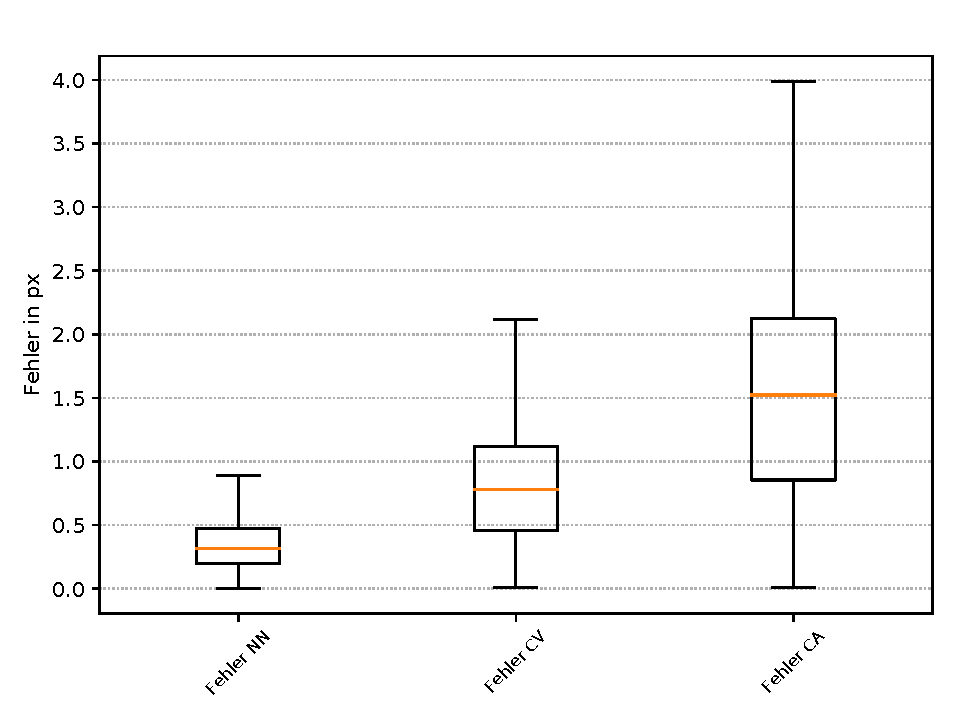
\includegraphics[width=\textwidth]{RealSpheres-evaluation_NextStep_LocationError_2018-12-10_18-42-20.pdf}
		\caption{Boxplots für die NextStep-Ergebnisse der selbst aufgenommenen Kugeln auf dem Förderband.}
		\label{subfig:RealSpheresBoxplot}
	\end{subfigure}
    % \quad
    \vskip\baselineskip
	\begin{subfigure}[t]{0.8\textwidth}
		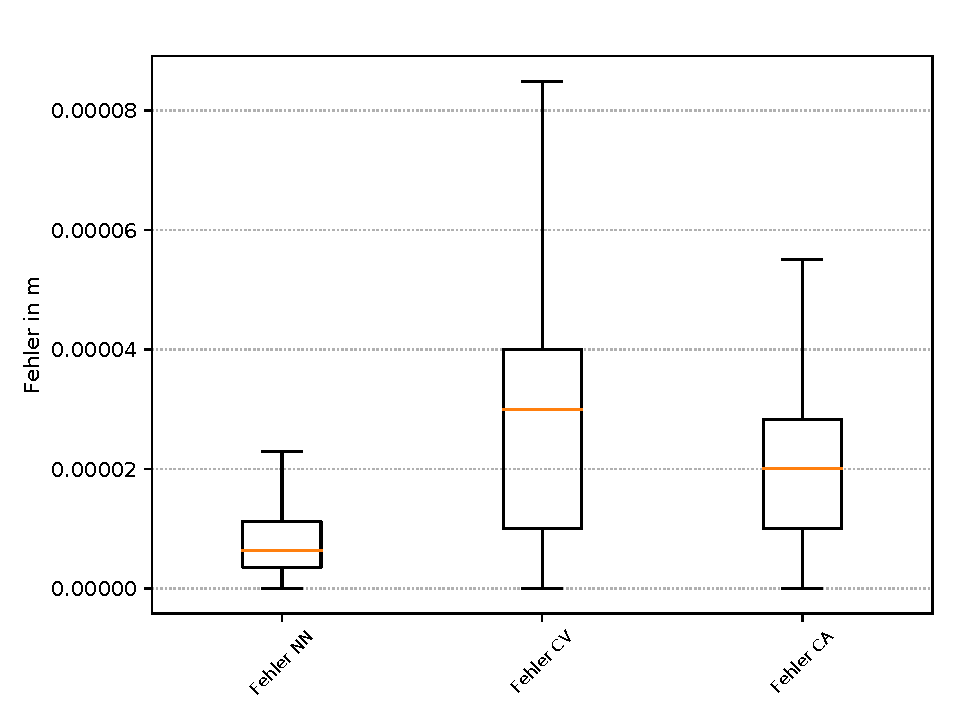
\includegraphics[width=\textwidth]{SimulatedSpheres-evaluation_NextStep_LocationError_2018-12-10_19-09-25.pdf}
		\caption{Boxplots für die NextStep-Ergebnisse der Kugeln aus dem DEM-Datensatz.}
		\label{subfig:SimSpheresBoxplot}
	\end{subfigure}
	
	\caption{Visualisierung der Ergebnisse }
	\label{fig:BoxplotsNextStep}
\end{figure}

\begin{figure}[h]
    \centering
    % \missingfigure{Boxplots Result NeuralNets NextStep}
	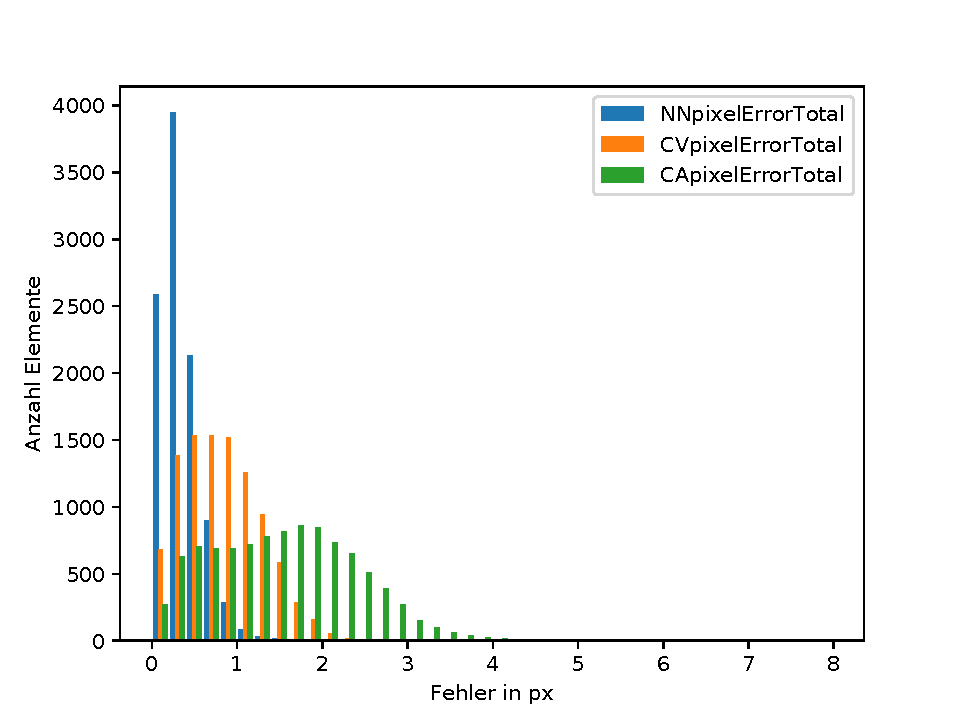
\includegraphics[width=0.8\textwidth]{RealSpheres-evaluation_NextStep_ErrorHistogram_2018-12-10_18-42-20.pdf}
	\caption{Histogramm der Fehler für die NextStep-Ergebnisse der selbst aufgenommenen Kugeln auf dem Förderband.}
	\label{fig:RealSpheresHistogram}
\end{figure}




% Bemerkenswert schlecht war das Ergebnis allerdings bei dem DEM Zylinder Datensatz.
% Es konnte nicht abschließend geklärt werden warum dies der Fall ist, vorallem da die Ergebnisse auf den realen Zylindern, wie in Abbildung TODO zu sehen, deutlich besser waren. 
% Man könnte jedoch vermuten, dass es eine Kombination der folgende Umstände ist.
% Bei den Zylindern hängt ihre Bewegung und die Aufnahme von Bewegungsenergie vom Förderband mehr von ihrer Orientierung ab, als bei den anderen Schüttgütern.
% Diese ist nicht aus den Eingabefeatures ersichtlich - potenziell wäre es bei diesem Szenario also lohnenswert mehr als nur die Mittelpunkte als Feature zu betrachten.
% Die höhere Bandgeschwindigkeit in der Simulation als in den Realdaten könnte diesen Effekt verstärkt haben.
% Auch könnte die höhere Schüttgutdichte auf dem Förderband darauf einen Einfluss gehabt haben.



\color{blue}
- CV, CA
- Ergebnis Netz

Vergleich Realdaten und simulierte Daten.
Realdaten mit ungefähr \SI{1.1}{\meter\per\second} während Simulierte mit \SI{1.5}{\metre\per\second} Bandgeschwindigkeit 

Zylinder schlechte performance erklären \textrightarrow orientierung fehlt?
\color{black}

\section{Separator}

\color{blue}
CV, CA quasi wie oben.
zusätzlich: CVBC, AA und IA

- Ergebnis NN
- Ergebnis Lineare Regression
\color{black}



In dieser Sektion sollen nun die Ergebnisse der Separator-Netze in verschiedenen Szenarien betrachtet und diskutiert werden.
Im Gegensatz zu diesen können die beiden Labelelemente nicht in einem gemeinsamen Evaluationskriterium zusammengefasst werden.
Deshalb werden hier die zeitliche Abweichung vom prädizierten Kontaktzeitpunkt mit dem Druckluftdüsenarray und die örtliche Abweichung des Schnittpunkts des Bahn des Partikels mit dem Druckluftdüsenarray separat betrachtet.
Ebenso wie bei den NextStep-Netzen werden hier ein Constant Velocity- und ein Constant Acceleration Modell als Vergleichsmodelle für die Ausgaben des neuronalen Netz benutzt.
Es werden mehr Vergleichsmodelle hinzugezogen. 
Das Bias-Corrected Constant Velocity Modell liefert eine sowohl Prädiktion für den Zeit als auch für den Ort.
Die Average Acceleration und Identical Acceleration Modelle werden nur für die zeitliche Prädiktion zum Vergleich herangezogen.

Die Evaluation, die hier durchgeführt wurde erfolg auf folgendem Szenario.
Als Trainingsdaten wurden nur das jeweils letzte Feature-Label-Paar eines Tracks benutzt, bevor das entsprechende Partikel die Prädiktionsphase verlässt.
Es wäre in der Zukunft möglich auf allen möglichen Feature-Label-Paaren zu trainieren um zu erreichen, dass der Ausgangspunkt verschoben werden kann ohne das Netz neu trainieren zu müssen.
\todo{Hier weg und dafür in den Ausblick?}  
Für die DEM Datensätze wurde von \(x = \SI{0.55}{\meter}\) nach \(x = \SI{0.70}{\meter}\) prädiziert, also \SI{15}{\centi\meter} nach vorne.
Da der gesamte Bildausschnitt der selbst aufgenommenen Daten weniger als \SI{15}{\centi\meter} entlang der Bewegungsrichtung misst musste diese Distanz reduziert werden.
Die letztendlich auf den selbst gesammelten Daten trainierten Netze prädizieren von \(y = \SI{800}{\px}\) nach \(y = \SI{1550}{\px}\), also eine Distanz von \SI{750}{\px}.


Die Ergebnisse auf den Separator-Netzen werden zweigeteilt als
\begin{align*}
    t\hitext{Err} &=  t\hitext{Pred} -  t\hitext{GT} \: ,\\
    \mathsf{y}\hitext{Err} &=  \mathsf{y}\hitext{Pred} -  \mathsf{y}\hitext{GT}
\end{align*}
definiert.
Im Gegensatz zu den NextStep-Netzen ist es nicht sinnvoll diese Fehler zu einem Gesamtfehler zu kombinieren.
Das Vorzeichen der Fehler für die einzelnen Partikel ist hier, ebenfalls im Gegensatz zu den NextStep-Netzen, angegeben.
Für die zeitlichen Fehler bedeutet ein positiver Wert also, 
dass das Teilchen früher den Druckluftdüsenarray passiert hat als von dem Modell vorhergesagt. 


Die Ergebnisse der neuronalen Netze für die Separator-Prädiktion sind insgesamt zufriedenstellend.
Sie sind auf allen Datensätzen besser als das Constant Velocity Modell, das Constant Acceleration Modell und das Bias-Corrected Constant Velocity Modell.
Auf den beiden simulierten Datensätzen sind die Ergebnisse ein wenig schlechter als das Identical Acceleration Modell, 
aber deutlich besser als die grundlegenden Modelle und dem Bias-Corrected Constant Velocity Modell.
Dies ist in Abbildung~\ref{fig:BoxplotsSimCub} exemplarisch durch die Boxplots der simulierten Plättchen dargestellt.

\begin{figure}[h]
    \centering
	
	\begin{subfigure}[t]{0.8\textwidth}
		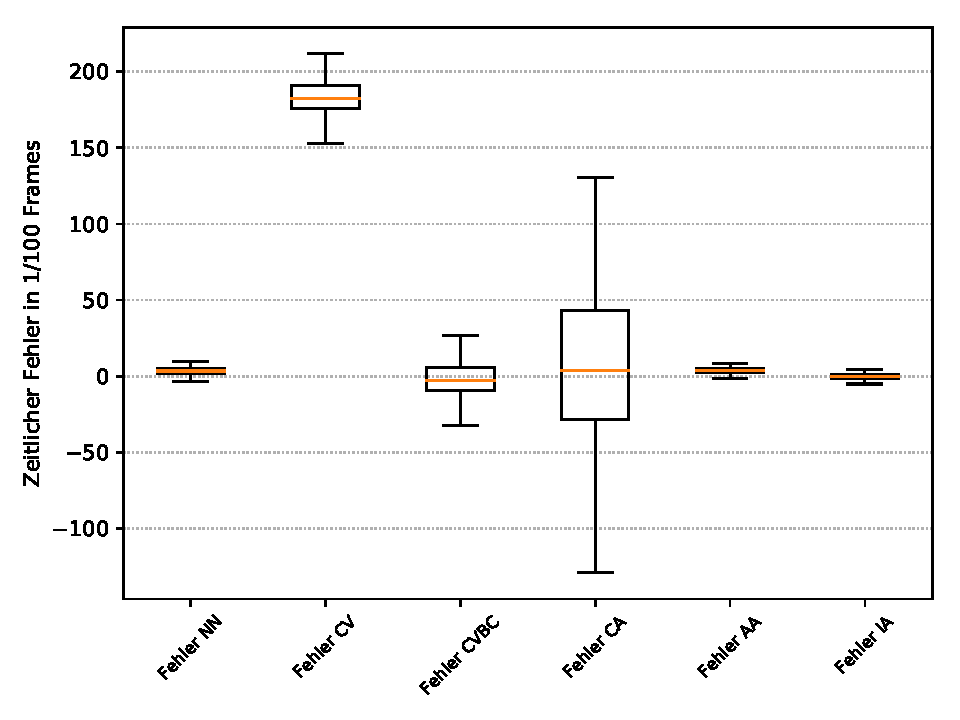
\includegraphics[width=\textwidth]{SimCub-evaluation_Separator_TimeErrorBoxplot_2018-12-11_14-33-22.pdf}
		\caption{Boxplots des zeitlichen Fehlers für die Separator-Ergebnisse der Plättchen aus dem DEM-Datensatz.}
		\label{subfig:SimCubTimeBoxplot}
	\end{subfigure}
    % \quad
    \vskip\baselineskip
	\begin{subfigure}[t]{0.8\textwidth}
		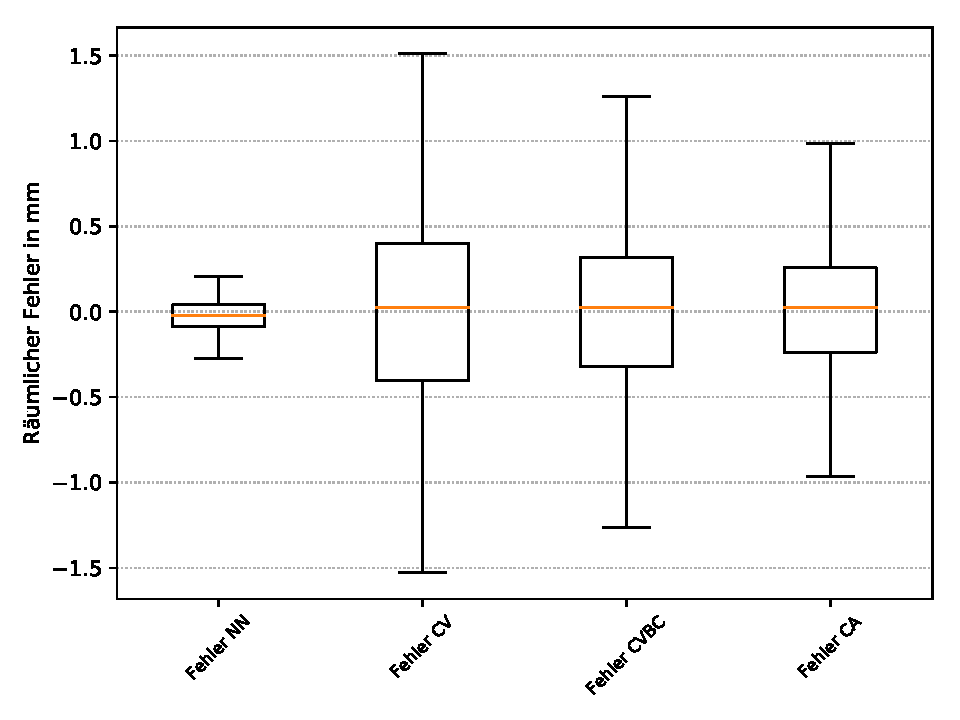
\includegraphics[width=\textwidth]{SimCub-evaluation_Separator_LocationErrorBoxplot_2018-12-11_14-33-22.pdf}
		\caption{Boxplots des örtlichen Fehlers für die Separator-Ergebnisse der Plättchen aus dem DEM-Datensatz.}
		\label{subfig:SimCubLocBoxplot}
	\end{subfigure}
	
	\caption{Visualisierung der Ergebnisse für die Plättchen aus der DEM-Simulation.}
	\label{fig:BoxplotsSimCub}
\end{figure}

Im Vergleich dazu sind die Unterschiede zwischen den verschiedenen Modellen auf den selbst aufgenommenen Daten deutlich kleiner.
Das Constant Velocity Modell, dessen mittlerer zeitlicher Fehler auf den DEM-Datensätzen einen signifikanten Bias gezeigt hat, schneidet oft beinah so gut 
und bei den Weizenkörnern, zu sehen in Abbildung~\ref{fig:BoxplotsRealWeizen}, sogar besser ab, als das Identical Acceleration Modell.
Auf den selbst gesammelten Daten schneidet von den bestehenden Modellen das Bias-Corrected Constant Velocity Modell am besten ab. 
Die neuronalen Netze sind jedoch [bis auf Pfeffer?] nocheinmal besser. 
\todo[inline]{Resultat verifizieren}
Dieses Resultat hängt höchstwahrscheinlich mit der niedrigeren Bandgeschwindigkeit und dem kürzeren Prädiktionsabstand zusammen.
Auch die könnten die unterschiedlichen Verfahren unterschiedlich anfällig gegen das Messrauschen sein, das ja auch den simulierten Daten nicht existiert.
Für die bestehenden Modelle gilt, dass eine relative Verbesserung der zeitliche Prädiktion zu einer Verbesserung der örtlichen Prädiktion führt, 
was besonders gut in Abbildung~\ref{fig:BoxplotsSimCub} zu erkennen ist, da die zeitliche Prädiktion benutzt wird um die örtliche zu treffen.
Für die Ausgabe der neuronalen Netze gilt das jedoch nicht. 

\begin{figure}[h]
    \centering
	
	\begin{subfigure}[t]{0.8\textwidth}
		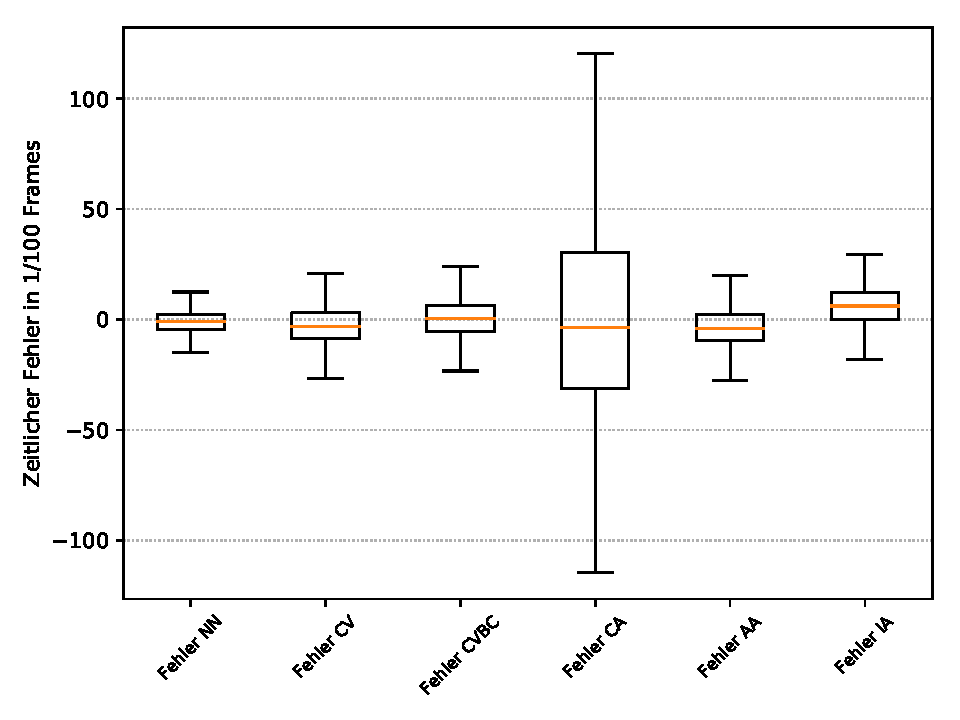
\includegraphics[width=\textwidth]{RealWeizen-evaluation_Separator_TimeErrorBoxplot_2018-12-11_14-09-12.pdf}
		\caption{Boxplots des zeitlichen Fehlers für die Separator-Ergebnisse des Weizenkörnern-Datensatz aus dem selbst gesammelten Datensatz.}
		\label{subfig:RealWeizenTimeBoxplot}
	\end{subfigure}
    % \quad
    \vskip\baselineskip
	\begin{subfigure}[t]{0.8\textwidth}
		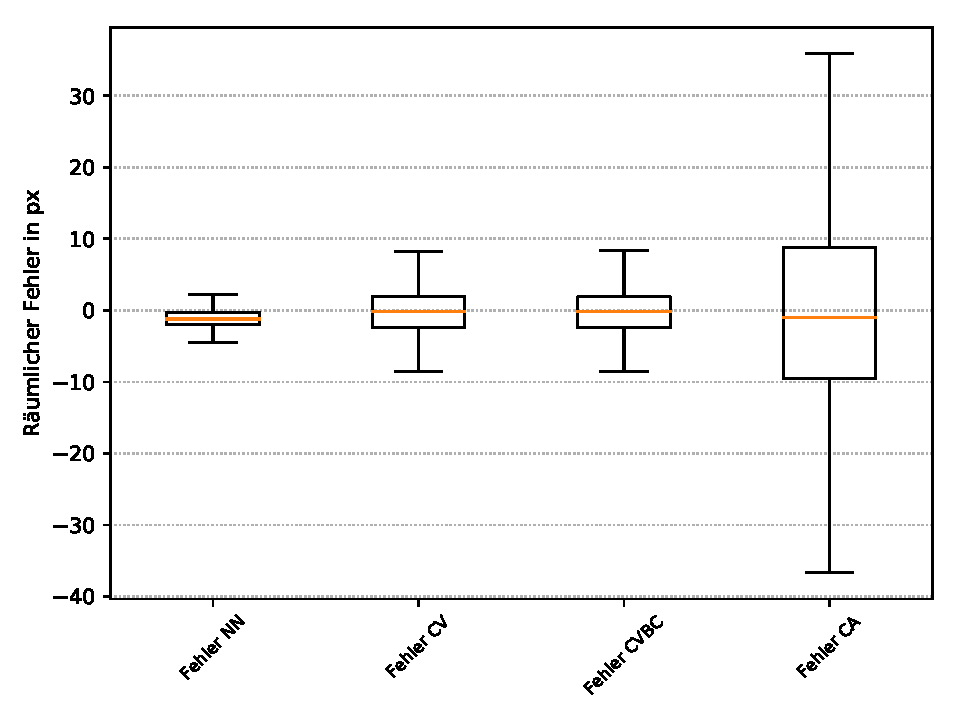
\includegraphics[width=\textwidth]{RealWeizen-evaluation_Separator_LocationErrorBoxplot_2018-12-11_14-09-12.pdf}
		\caption{Boxplots des örtlichen Fehlers für die Separator-Ergebnisse des Weizenkörnern-Datensatz aus dem selbst gesammelten Datensatz.}
		\label{subfig:RealWeizenLocBoxplot}
	\end{subfigure}
	
	\caption{Visualisierung der Ergebnisse für den Weizenkörnern-Datensatz aus dem selbst gesammelten Datensatz.}
	\label{fig:BoxplotsRealWeizen}
\end{figure}

Wie schon für die NextStep-Netze sind die Boxplots und Histogramme der restlichen Szenarien im Anhang zu finden.

\section{Zusammenfassung und Diskussion}


Die Fehlerfunktion nach der die neuronalen Netze optimiert worden ist, ist die MSE-Funktion.
Es konnte beobachtet werden, dass bei mehrmaligem Trainieren eines Netzes 
mit identischen Hyperparametern und Daten, unterschiedliche Ergebnisse mit einem ähnlichen MSE insgesamt aber einer Verschiebung zwischen dem Mittelwert und der Standardabweichung  
an dessen Ende standen.
Für die Separator-Netze kam es sogar zu Verschiebungen zwischen der örtlichen und der zeitlichen Prädiktion.
Dies ist auf verschiedene stochastische Vorgänge während dem Training zurück zu führen, wie die Initialisierung der Gewichte zwischen den Neuronen und die Reihenfolge beziehungsweise das Batching der Trainingsbeispiele.
Der Einsatz einer anderen Fehlerfunktion, zum Beispiel [einer die tatsächlich Richtig/Falsch Sortiert bewertet] könnte dieses Problem beheben.

    \chapter{Fazit und Ausblick}
\label{cap:fazit}
% \todo[inline]{einführungstext in Fazit und Ausblick}

Im Rahmen dieser Arbeit wurde betrachtet, ob neuronale Netze ein Werkzeug sind, das für die Bewegungsprädiktion von Schüttgutpartikeln eingesetzt werden kann.
Dazu wurden zunächst beinahe 250\,000 Bilder von verschiedenen Schüttgütern auf dem \textit{TableSort}-Schüttgutsortierer aufgenommen 
und eine Pipeline entwickelt, mit der die relevanten Features aus solchen Bildern extrahiert werden können.
Zusätzlich wurde eine einfache Form der Datenaugmentierung implementiert, die die Menge an verfügbaren Trainingsdaten für die jeweiligen Datensets beinahe verdoppelt.
Es wurde mit Hilfe des TensorFlow Frameworks eine Implementierung erarbeitet, mit der verschiedene neuronale Netze trainiert werden können.
Mit dieser Implementierung wurden mehrere Netze auf verschiedenen Datensets trainiert -- den selbst aufgenommenen und bereits existierenden, mittels DEM simulierten -- und deren Ergebnisse evaluiert.
Es wurde festgestellt, dass die Bewegungsprädiktion von Schüttgutpartikeln eine Aufgabe ist, für die neuronale Netze geeignet sind.
Es konnte gezeigt werden, dass sowohl NextStep-, als auch Separator-Netze gut in der Lage sind, die an sie gestellten Probleme zu lösen.
In jedem Szenario konnten Ergebnisse erzielt werden, die besser als die der zwei grundlegenden Bewegungsmodelle
und vergleichbar mit dem aktuellen Stand der Technik waren.
Insbesondere auf den Datensätzen, die auf realen Aufnahmen basieren, wurden die Ergebnisse des aktuellen Stands der Technik übertroffen.
% Dies gelang, obwohl das manuelle Hyperparameter-Tuning auf den simulierten Datensätzen durchgeführt wurde.


% \todo[inline]{blick darauf wie es gelaufen ist...}

% Mehr daten für separator!\\
% Zylinder war eher so Meh, da ist noch ausbaupotenzial.

% \todo[inline]{was man noch so machen könnte...}

In dieser Arbeit wurde nur ein Ansatz für den Einsatz von neuronalen Netzen für die Bewegungsprädiktion von Schüttgutpartikeln erprobt.
Obwohl positive Ergebnisse erzielt wurden, gibt es noch viele weitere vielversprechende Ansätze, die es wert sind, betrachtet zu werden.
Naheliegende Ideen wären zum Beispiel alternative Modellierungen, wie die Verwendung relativer Positionen als Eingabe statt absoluter, 
oder zusätzliche Features, die zu den existierenden Objektmittelpunkten hinzugekommen.
Beispielsweise ein zusätzliches Feature, das die Orientierung des Partikels beschreibt, würde speziell bei den Schüttgutsorten Zylinder und Weizenkörner Sinn ergeben.
Auch ist denkbar, dass der Einsatz anderer Netzwerkarchitekturen für Verbesserungen sorgen könnte. 
Rekurrente neuronale Netze sind besonders gut dafür geeignet, Daten, bei denen die zeitliche Abfolge wichtig ist, sequenziell zu verarbeiten.

Maschinelles Lernen allgemein und neuronale Netze im Besonderen sind ein Feld, auf dem momentan sehr schnell große Fortschritte gemacht werden,
die in naher Zukunft vielleicht ganz neue Möglichkeiten eröffnen werden.
Heutige Möglichkeiten sind auch noch nicht ausgereizt.
Ein Aspekt, in dem neuronale Netze schon jetzt beindruckende Ergebnisse liefern, ist das Extrahieren von Informationen direkt aus Bildern.
Es gibt bereits heute Multi-Object-Tracking Verfahren, die sehr gute Ergebnisse erzielen. 
Beispiele hierfür sind \cite{Milan2017}, \cite{son2017multi} und \cite{ning2017spatially}.
% \todo{hier eine Quelle?}
Deshalb liegt es nahe, dass es möglich sein sollte, auf den Bildern direkt Ende-zu-Ende zu trainieren.
Das könnte dabei helfen Ungenauigkeiten und Fehler, die während der in Abschnitt~\ref{sec:pipeline} beschriebenen Datenpipeline entstehen, zu vermeiden.
% Das würde unter anderem das Problem von Messunsicherheiten bei der Bestimmung der Objektmittelpunkte irrelevant machen.

% \todo{hier anmerken, dass das wahrscheinlich ein größeres Projekt wäre und mehr als nur ne MA?}
Sowohl im aktuellen Stand der Technik als auch bei den im Rahmen dieser Arbeit trainierten Netzen werden alle Schüttgutpartikel individuell betrachtet.
Dies führt dazu, dass Kollisionen zwischen Partikeln, die diese von ihrer Bahn ablenken höchstens detektiert, aber nicht sinnvoll in die Modelle miteinbezogen werden können.
Ein Ansatz, der dies tut, könnte insbesondere für Schüttgüter mit einer starken Querbewegung zu einer Verbesserung der Sortierqualität führen.


% Ende zu Ende lernen: Sollte das Problem mit dem segmentieren lösen, das ich hatte
% (Sprengt aber vielleicht den Rahmen einer MA)\\
% Orientierung als Feature, das man noch reinnehmen könnte?\\
% Lernen während dem laufenden Betrieb?\\
% Mehrere Partikel gleichzeitig betrachten? Irgendwie mit Kollisionen umgehen


    % \nocite{*}
	\cleardoublepage
	\phantomsection
	\addcontentsline{toc}{chapter}{Literatur}
    \printbibliography %[heading=bibintoc]


    \appendix
    \chapter{Anhang}

Hier ist der Anhang. Hier kommen Dinge Rein, wie Evaluationsergebnisse, 
die den Hauptteil zu voll machen würden, Tabellen mit daten, die nur begrenzt was mit der Arbeit zu tun haben,


% Please add the following required packages to your document preamble:
% \usepackage{booktabs}
% Please add the following required packages to your document preamble:
% \usepackage{booktabs}



\end{document}

